\documentclass[a4paper,12pt]{article}

\usepackage{hyperref}
\usepackage[all]{xy}
\usepackage[english]{babel}
\usepackage[margin=1in]{geometry}
\usepackage[utf8]{inputenc}
\usepackage{amsmath}
\usepackage{mathtools}
\usepackage{amsthm}
\usepackage{amsfonts}
\usepackage{graphicx}
\usepackage{amssymb}
\usepackage{arydshln}
\usepackage{booktabs}
\usepackage[colorinlistoftodos]{todonotes}
\usepackage{tikz}
\usepackage{pgfplots}
\usepackage{tikz}
\usetikzlibrary{matrix,arrows,decorations.pathmorphing}
\usepackage{soul}
\usepackage{float}
\usepackage{framed, color}
\usepackage[normalem]{ulem}


% preamble
\newtheorem{remark}{Remark}[section]
\newtheorem{lemma}{Lemma}[section]
\newtheorem{theorem}{Theorem}[section]
\newtheorem*{lemma*}{Lemma}
\newtheorem{proposition}{Proposition}[section]
\newtheorem{definition}{Definition}[section]
\newtheorem{question}{Question}[section]
\newtheorem{example}{Example}[section]
\newtheorem{Corollary}{Corollary}[section]
\newtheorem{claim}{Claim}[section]
\newcommand{\tr}{\mathrm{tr}}
\newcommand{\mc}{\mathcal{M}^{\mathrm{mc}}}
\newcommand{\mcrl}{\mathcal{M}^{\mathrm{mc}}_{rl}}
\newcommand{\mm}{\mathcal{M}^{\mathrm{w}}}
\newcommand{\fmm}{\mathcal{M}^{\mathrm{w}}_{f}}
\newcommand{\dotcup}{\ensuremath{\mathaccent\cdot\cup}}

\newcommand{\no}{\noindent\textbf}


%%%%%%%%%%
\definecolor{darkblue}{rgb}{0.0, 0.0, 0.8}
\definecolor{darkred}{rgb}{0.8, 0.0, 0.0}
\definecolor{darkgreen}{rgb}{0.0, 0.8, 0.0}

\newcommand{\woojin}[1]           {{ \textcolor{darkblue} {#1}}}
\newcommand{\facundo}[1]                {{ \textcolor{darkred} {#1}}}
\newcommand{\zane}[1] 			{{ \textcolor{darkgreen} {#1}}}

%%%%%%%%%%

\makeatletter
\def\moverlay{\mathpalette\mov@rlay}
\def\mov@rlay#1#2{\leavevmode\vtop{%
   \baselineskip\z@skip \lineskiplimit-\maxdimen
   \ialign{\hfil$\m@th#1##$\hfil\cr#2\crcr}}}
\newcommand{\charfusion}[3][\mathord]{
    #1{\ifx#1\mathop\vphantom{#2}\fi
        \mathpalette\mov@rlay{#2\cr#3}
      }
    \ifx#1\mathop\expandafter\displaylimits\fi}
\makeatother

\newcommand{\cupdot}{\charfusion[\mathbin]{\cup}{\cdot}}
\newcommand{\bigcupdot}{\charfusion[\mathop]{\bigcup}{\cdot}}




\newcommand{\eps}{\varepsilon}
\newcommand{\met}{\mathcal{M}}


\newcommand{\dgm}{\mathrm{dgm}}

\newcommand{\C}{\mathrm{C}}

\newcommand{\length}[1]{\mathrm{length}(#1)}


\newcommand{\prob}{\mathcal{P}}
\usepackage{mathtools}
\DeclarePairedDelimiter{\abs}{\lvert}{\rvert}
\newcommand{\Expect}{{\rm I\kern-.3em E}}
\newcommand{\norm}[1]{\left\lVert#1\right\rVert}
\newcommand{\hookuparrow}{\mathrel{\rotatebox[origin=c]{90}{$\hookrightarrow$}}}
\newcommand{\hookdownarrow}{\mathrel{\rotatebox[origin=c]{-90}{$\hookrightarrow$}}}


\title{Formigrams: Clustering Summaries of Dynamic Data}
%\title{Clustering of Directed Data}

\author{ W. Kim, F. M\'emoli, Z. Smith}

\date{\today}

\begin{document}
\maketitle
\begin{center}
\textbf{Outline}
\end{center}

\begin{itemize}
\item[1] Introduction to formigrams: Definitions of formigrams, grouping functions, recovery of formigrams from grouping/\facundo{flocking}/
\facundo{swarming} \facundo{collective behavior.} functions.\footnote{\url{https://en.wikipedia.org/wiki/Swarm_behaviour}. We should choose a suggestive name here.} \woojin{swarming function or swarm function would be nice in my opinion. Choose as you want and please let me know.}

\item[2] Persistence diagrams derived from linearization. 

\item[3] Set theoretic persistence diagrams: %\facundo{Discuss the feature that we work with triples $(X,\theta_X,\mathfrak{o}_X).$}
\begin{itemize}
\item[3.1] Order on Underlying set and New Diagrams: \woojin{some useful definitions by assigning an order \& the Def of set-theoretic diagram.}
\item[3.2] The Relationship Between The Set-Theoretical Persistent Diagrams and Original Persistent Diagrams 
\begin{itemize}
\item[3.2.1] Case of Dendrograms; \woojin{Proof for set-theoretic diagram=original diagram}
\item[3.2.2] Case of Formigramss; \woojin{Proof for set-theoretic diagram $\neq$ original diagram by providing an example having two different set-theoretic diagrams depending on orders. Also, we can study more on the relation between the set-theoretic persistent diagram and algebraic persistent diagram here.}
\end{itemize}
\end{itemize}
\item[4] Stability Results for Dendrograms. \woojin{Proof for $2\ \mathrm{dist}(\theta_X, \theta_Y)\geq d_B(\dgm(\theta_X), \dgm(\theta_Y))$ when $\theta_X$ and $\theta_Y$ are dendrograms. The diagram on RHS is algebraic persistent diagram.}

\item[5] Stability Results for Formigrams.
\begin{itemize}
\item[5.1] Stability results for set-theoretic persistent diagrams. %\facundo{The metric dist between triples $(X,\theta_X,\mathfrak{o}_X)$\& Stability theorem for  set theoretic formigrams. All details.} 
\begin{itemize}
\item[5.1.1] Groundwork \woojin{Isometry theorem for intervals systems: For all intervals' systems $\mathcal{A}$ and $\mathcal{B}$, \ \  $d_H^\mathbb{R}(C(\mathcal{A}),C(\mathcal{B}))=d_B(\mathcal{A},\mathcal{B})$}
\item[5.1.2] Stability results \woojin{Proof for $2\  \mathrm{dist}_{\mathfrak{O}}(\mathcal{X},\mathcal{Y})\geq d_B(\dgm(\mathcal{X}), \dgm(\mathcal{Y}))$}
\end{itemize}

\item[5.2] Stability results for algebraic persistent diagrams.
\begin{itemize}
	\item[5.2.1] Computing the algebraic persistent diagram of planar formigrams \woojin{I introduce the algorithm the compute the algebraic diagram of planar formigram.}
	\item[5.2.2] Relationship between the set-theoretic diagrams and the algebraic diagrams
\end{itemize}



\end{itemize}


\item[6] Computational details and experiments.

\item[7] Curves on the space of metric spaces
\end{itemize}

\medskip

\begin{center}
\textbf{References}
\end{center}

\url{http://link.springer.com/chapter/10.1007%2F978-3-642-33042-1_60}

\url{https://math.la.asu.edu/~helene/papers/blsocialjan06.pdf
}



\newpage

\section{Introduction to Formigrams}

The goal is to construct the theoretical frame work for dendrogram-like structure illustrating the clustering information of time-varying graphs or point clouds.

Let $X$ be a non-empty finite set. The collection of partitions $\mathcal{P}(X)$ is regarded as a category whose objects are partitions and arrows $\leq$ mean the relation 'is finer than'. Especially, we shall use $<$ to indicate the phrase 'is finer than and not identical to' from now on.

\subsection{Review of Dendrograms}
 To say that $\theta_X=\{\theta_X(t)\in \mathcal{P}(X)\}_{t\in\mathbb{R}^+}
$ is a dendrogram means that the following properties hold:

\begin{itemize}
\item $\theta_X(0)=\{\{x\}: x\in X\}$
\item If $t_1\leq t_2$, then $\theta_X(t_1) \leq \theta_X(t_2)$.
\item There exists $T\geq0$ such that and $\theta_X(t)=\{X\}$ for $t\geq T$.
\item For all $t$ there exists $\epsilon>0$ s.t. $\theta_X(s)=\theta_X(t)$ for $s\in [t,t+\epsilon]$. (technical condition)

\end{itemize}

Note that dendrogram natually yields a metric on the underlying set, which in turn makes it possible to measure the distance between two dendrograms. Denote a collection of the closed subsets of $\mathbb{R^+}$ by $Closed(\mathbb{R^+})$.
\begin{definition} Define $t_{\theta_X}:X\times X \rightarrow Closed(\mathbb{R}^+)$ by 
$$t_{\theta_X}(x,x')=\{t\in \mathbb{R}^+|\ x, x'\ \mbox{belong to the same block of}\ \theta_{X}(t)\}$$
\end{definition}

Observe that $t_{\theta_X}=[\alpha, \infty)$ for some $\alpha >0$ for any $x,x'\in X$. So we define $\mathcal{U}_{\theta_X}(x,x')=\alpha$ and this is an ultrametric on $X$. This mean that for all $x,x',x''\in X$ one has $$\mathcal{U}_{\theta_X}(x,x'')\leq \max\big\{\mathcal{U}_{\theta_X}(x,x'),\mathcal{U}_{\theta_X}(x',x'')\big\}.$$


\begin{definition} Let $X$, $Y$ be sets and $\theta_X$, $\theta_Y$ be dendrograms on $X$ and $Y$ respectively. The distance between to dendrograms is defined as follows:\label{dist}

\begin{align*}
\mathrm{dist}(\theta_X, \theta_Y)&=d_{GH}((X,\mathcal{U}_{\theta_X}),(Y,\mathcal{U}_{\theta_Y}))\\&= \frac{1}{2}\inf_{R\in\mathcal{R}(X,Y)}\max_{(x,y)\in R, (x'y')\in R}\abs{\mathcal{U}_{\theta_X}(x,x')-\mathcal{U}_{\theta_Y}(y,y')}
\end{align*}
\end{definition} 
\begin{remark}Observe that $$\abs{\mathcal{U}_{\theta_X}(x,x')-\mathcal{U}_{\theta_Y}(y,y')}=d_{H}^{\mathbb{R}}(t_{\theta_X}(x,x'), t_{\theta_Y}(y,y'))$$
\end{remark}
Though dendrogram is useful notion to represent clustering process, we also need more flexible concept allowing 'refining' of partition in order to illustrate diverse clustering behavior of dynamic data or graphs.



\subsection{Formigrams}
Here we suggest the notion of zigzag-dendrogram as below. The name \emph{formigram} is a mixed word using formicarium and dendrogram in accordance with its shape of pictorial expression.
\begin{definition} (Formigram)
To say that $\theta_X=\{\theta_X(t)\in \mathcal{P}(X)\}_{t\in\mathbb{R}}
$ is a formigram means that there exists a finite set $C=\{c_1< c_2< \cdots< c_n\} \subset \mathbb{R}$ such that

\begin{itemize}
\item[1.] Either $\theta_X(c_i-\epsilon) <\theta_X(c_i)$ or $\theta_X(c_i-\epsilon) > \theta_X(c_i)$  for all $1 \leq i \leq n$ and small enough $\epsilon>0$. 

\item[2.] If $t_1$, $t_2$ belong to the same connected component of $(-\infty, c_1)\dotcup [c_1, c_2) \dotcup \cdots \dotcup [c_n,\infty)$, then $\theta_X(t_1)=\theta_X(t_2)$.
%\item[3.] (Distinction) For pair $x,x'\in X$, there is a time $t$ when they are contained in the different blocks. 
\item[3.](Impermanence) $\theta_X(t)=\{X\}$ for $t\in (\infty, c_1)\dotcup [c_n,\infty)$. \label{def}
\end{itemize}
We call the elements of $C$ critical points of the formigram $\theta_X$.
\end{definition}


\woojin{I have deleted "Distinction" condition in the original definition}
%\woojin{The reason I added the 3rd condition was only to define a proper metric $d_{\theta_X}(x,x')=\mathrm{length}(\mathbb{R}\setminus t_{\theta_X}(x,x'))$ on $X$ from the formigram $\theta_X$. Shall we delete it? Or Keep it? Do we contain the definition of $d_{\theta_X}$ in this document?}

\begin{remark} This definition is a relaxation of the notion of dendrogram after trivial modification: a dendrogram satisfies all the axiom stated above except the 3rd condition, which is essential difference between formigrams and dendrograms. 

\end{remark}



\begin{definition}(Grouping function) Define $t_{\theta_X}:X\times X \rightarrow \mathrm{Int}(\mathbb{R}\cup \{-\infty\})$ by 
$$t_{\theta_X}(x,x'):=\{t\in \mathbb{R}|\ x, x'\ \mbox{belong to the same block of}\ \theta_{X}(t)\}$$
where $\mathrm{Int}(\mathbb{R}\cup \{-\infty\})$ is the collection of the finite unions of half-open intervals of the form $[a,b)$.
\end{definition}

\begin{definition} Let $\theta_X$ be a formigram.  Define $t_{\theta_X}:X\times X \rightarrow \mathrm{Pow}(\mathbb{R})$ by 
$$t_{\theta_X}(x,x'):=\{t\in \mathbb{R}|\ x, x'\ \mbox{belong to the same block of}\ \theta_{X}(t)\}$$
\end{definition}
Note that $t_{\theta_{X}}(x,x')=(-\infty, -T]\cup \dot{\bigcup}_i{[a_i, b_i)} \cup [T, \infty)$ for a finite sequence of real numbers $-T \leq a_1<b_1<\cdots<a_n<b_n\leq T$. Especially, $t_{\theta_X}(x,x)=\mathbb{R}$ for all $x\in X$.

\begin{remark}
Similarly to the ultrametric property, we now have for any formigrams $\theta_X$ that for all $x,x',x''\in X$ it holds that 
$$t_{\theta_X}(x,x')\cap t_{\theta_X}(x',x'')\subseteq t_{\theta_X}(x,x'').$$
\begin{proof}
Let $r\in t_{\theta_X}(x,x')\cap t_{\theta_X}(x',x'')$. This fact indicates that not only $x$ and $x'$ belong to the same block at time $r$ but  also $x'$ and $x''$ are included in the same block at the same time $r$. Therefore, $x$ and $x''$ belong to the same block at time $r$ and $r\in t_{\theta_X}(x,x'')$ as desired.
\end{proof}
\end{remark}

\begin{definition} Let $X$, $Y$ be sets and $\theta_X$, $\theta_Y$ be formigrams on $X$ and $Y$ respectively. The distance between to two formigrams is defined as follows:\label{dist2}

\begin{align*}
\mathrm{dist}(\theta_X, \theta_Y)= \frac{1}{2}\inf_{R\in\mathcal{R}(X,Y)}\max_{(x,y)\in R, (x'y')\in R}d_{H}^{\mathbb{R}}(t_{\theta_X}(x,x'), t_{\theta_Y}(y,y'))
\end{align*}
Note that this definition coincides with Definition \ref{dist} in the case where $\theta_X$ and $\theta_Y$ are dendrograms.
\end{definition} 



\begin{definition}(Pullback of partition) Let $X,Y$ be two sets, $\varphi:X\rightarrow Y$ a map and $P\in \mathcal{P}(Y)$. Then 
$\varphi^*P\in \mathcal{P}(X)$ is defined by

$$\varphi^*P=\{\varphi^{-1}(U): U\in P\}.$$
\end{definition}

\facundo{below we probably need to make sure that the pullback really is a formigram according to our definition of fomrigram.}\woojin{OK}

\begin{definition}\label{pullback}(Pullback of formigram) Let $X$ be a set and $\theta_Y$ be a formigram on a set $Y$. Let $\varphi:X\rightarrow Y$ be a map. Then the formigram $\varphi^*\theta_Y$ is defined by
$$\varphi^*\theta_Y=\{\varphi^*\theta_Y(t)\in \mathcal{P}(X)\}_{t\in\mathbb{R}}$$
\end{definition}

\begin{proposition} The previous definition is well-defined.
\begin{proof}
\woojin{elaborate}
\end{proof}

\end{proposition}



The following proposition suggests that a grouping function is equivalent to a formigram.
\begin{proposition} Let $X$ be a non-empty finite set. Any function $f:X\times X \rightarrow \mathrm{Int}(\mathbb{R}\cup\{-\infty\})$ satisfying the following conditions define a formigram.
\begin{itemize}
\item[1.] (Reflexivity) For any $x\in X$, $f(x,x)=\mathbb{R}$ 
\item[2.] (Symmetry) For any $x,x'\in X$, $f(x,x')=f(x',x)$
\item[3.] (Transitivity) For any $x,x',x''\in X$, $f(x,x')\cap f(x',x'')\subseteq	 f(x,x'')$

\item[4.] (Continuity and Impermanence) For any $x,x'\in X$, $f(x,x')=(-\infty, -T]\cup \dot{\bigcup}_i{[a_i, b_i)} \cup [T, \infty)$ for a finite sequence of real numbers $-T \leq a_1<b_1<\cdots<a_n<b_n\leq T$

\end{itemize}
 
\begin{proof} For each $t\in \mathbb{R}$, we shall define an  equivalence relation $\sim_{t}$ on $X$, which amounts to defining a partition on $X$, as follows: $$x\sim_t x' \Leftrightarrow t\in f(x,x').$$   

The first three conditions on $f$ guarantees the $\sim_t$ to be an equivalence relation on $X$. Divide the cases into '$t=a_i$ or $t=b_i$'and the other.\woojin{Will be proven later. By the way, do we need this proposition really? I believe this proposition is true but the proof will be not short.}

\end{proof}
\end{proposition}

\section{Persistence Diagrams Derived from Linearization}

\begin{definition} Let $X$ be a set and $\theta_X$ be a dendrogram/formigram on $X$. For each $t\in \mathbb{R}$, the block containing $x\in X$ is denoted by $[x]_t$. 
\end{definition}

\begin{definition}(Persistent Diagram for dendrogram) Let $\theta_X$ be a dendrogram on $X$ with critical values $0=c_0<c_1< c_2< \cdots <c_n$ Let $c_{n+1}=\infty$ and $V_{n+1}=\mathrm{Lin}(\{X\})\approx \mathbb{R}$. Consider a persistence module $\mathcal{V}$ of length $n+2$ in \textbf{Vect} defined as follows: For each $i=0, 1, 2,\cdots, n$, let $V_i=\mathrm{Lin}(\theta_X(c_i))$. Also, define  $T_{i-1}:V_{i-1}\rightarrow V_{i}$ by $[x]_{c_{i-1}}\mapsto [x]_{c_{i}}$.

By Gabriel's theorem, $\mathcal{V}$ can be decomposed as a direct sum of intervals $\mathbb{I}(b,d)$ where $b,d$ are non-negative integers. We define $\dgm(\theta_X)$ by the multiset consisting of such intervals $[c_b,c_{d+1})$. \label{diagram0}
\end{definition}

\begin{remark} The set $\{0=c_0, c_1, \cdots, c_n\}$ of critical points in the above definition is identical to $\mathrm{Spec}(\mathcal{U}_{\theta_X})=\{\mathcal{U}_{\theta_X}(x,y): x,y\in X\}$ where $\mathcal{U}_{\theta_X}$ is the ultrametric induced by the dendrogram $\theta_X$.

\end{remark}

\begin{definition}(Persistent Diagram for formigram) Let $\theta_X$ be a formigram on $X$ with critical values $c_1< c_2< \cdots <c_n$. Let $c_0=-\infty$ and $c_{n+1}=\infty$ and $V_{0}=V_{n+1}=\mathrm{Lin}(\{X\})\approx \mathbb{R}$. Consider a zigzag module $\mathcal{V}$ of length $n+2$ in \textbf{Vect} defined as follows: For each $i=1, 2,\cdots, n$, let $V_i=\mathbb{F}(\theta_X(c_i))$. Also, define  
\begin{itemize}
\item[] $T_{i}:V_{i}\rightarrow V_{i+1}$ by $[x]_{c_{i}}\mapsto [x]_{c_{i+1}}$ if $\abs{\theta_X(c_{i})}\geq\abs{\theta_X(c_{i+1})}$

\item[] $S_{i}:V_{i+1}\rightarrow V_{i}$ by $[x]_{c_{i+1}}\mapsto [x]_{c_{i}}$ if $\abs{\theta_X(c_{i})}<\abs{\theta_X(c_{i+1})}$

\end{itemize}
By Gabriel's theorem, $\mathcal{V}$ can be decomposed as a direct sum of intervals $\mathbb{I}(b,d)$ where $b,d$ are non-negative integers. We define $\dgm(\theta_X)$ by the multiset consisting of such intervals $[c_b,c_{d+1})$. \label{diagram} \footnote{The reason to define $\dgm(\theta_X)$ will become clear later.}
\end{definition}

%\woojin{We have the following alternative choice for the persistent diagram; If we adopt the definition below, then I have some ideas to compute persistent diagram and relate it to the set-theoretic diagram though still the idea is not completely tested.}

%\begin{definition}(Alternative Persistent Diagram) Let $\theta_X$ be a formigram on $X$ with critical values $c_1< c_2< \cdots <c_n$. Let $c_0=-\infty$ and $c_{n+1}=\infty$ and $V_{0}=V_{n+1}=\mathrm{Lin}(\{X\})\approx \mathbb{R}$. Consider a \textbf{persistent} module $\mathcal{V}$ of length $n+2$ in \textbf{Vect} defined as follows: For each $i=0, 1, 2,\cdots, n$, let $V_i=\mathrm{Lin}(\theta_X(c_i))$. Also, define linear maps $T_{i}:V_{i}\rightarrow V_{i+1}$ by \begin{equation*}A \mapsto \sum_{j=1}^k \mathbf{1}_{A\cap B_{j}} B_{j}\end{equation*} for all $A\in \theta_X(c_{i})$ where $\theta_X(c_{i+1})=\{B_j\}_{j=1}^{k}$ and $\mathbf{1}_{A\cap B_{j}}$ is the indicator function of the set $A\cap B_{j}$ for each $j$. Then $\mathcal{V}$ is decomposed as a direct sum of intervals $\mathbb{I}(b,d)$ where $b,d$ are non-negative integers. We define $\dgm(\theta_X)$ by the multiset consisting of such intervals $[c_b,c_d+1)$. \label{diagram}\end{definition}

\begin{remark} Two definitions coincide in the case of dendrograms.(But, in the case of dendrogram, the minimum critivcal value is 0 and hence $V_0=\mathbb{F}\big(\theta_X(0))\big)=\mathbb{F}\Big(\big\{\{x\}: x\in X\big\}\Big)$
\end{remark}

\begin{proposition}
Let $\theta_X$ be a dendrogram on $X$ with critical values $0=c_0<c_1< c_2< \cdots <c_n$.
Then, $\dgm(\theta_X)$ is the multiset containing $[0,c_i)$ for all $1\leq i\leq n$ with $\#[0,c_i)=\abs{\theta_X(c_{i-1})}-\abs{\theta_X(c_i)}$.
In words, we can compute a barcode by looking at the variation of the cardinality of partitions at each critical point. 
\label{dgm2}
 
\begin{proof} We follow Definition \ref{diagram0}. Consider a persistent module $\mathcal{V}$ in \textbf{Vect} and let $V_i=\mathrm{Lin}(\theta_X(c_i))$ and $T_i:V_i\rightarrow V_{i+1}$ a linear map defined by $T_i([x]_{c_i})=[x]_{c_{i+1}}$ for each $0\leq i \leq n-1$ and $x\in X$. Then we obtain a tower in $\mathbf{Vect}$ as below.
 
$$\mathcal{V}:=V_0\xrightarrow[]{T_0}  V_1 \xrightarrow[]{T_1} \cdots \xrightarrow{T_{n-3}} V_{n-2}\xrightarrow{T_{n-2}} V_{n-1} \xrightarrow{T_{n-1}} V_n$$

Note that $\#[c_i,c_j)(\mathcal{V})=T_i^{j-1}-T_{i-1}^{j-1}-T_i^{j}+T_{i-1}^{j}$ where $T_i^j$ stands for $\mathrm{rank}(T_j \circ \cdots \circ T_{i+1}\circ T_i)$ for all $0\leq i < j \leq n$. However, $T_i^{j-1}=T_{i-1}^{j-1}=\dim(V_{j-1})$ and $T_i^{j}=T_{i-1}^{j}=\dim(V_{j})$ for all $i\geq1$ because $T_i$ is surjective for each $i$ in the case we are dealing with. Therefore, $\#[c_i,c_j)(\mathcal{V})=0$ for every $i\geq 1$. Now let $i=0$. Then $\#[0,c_j)(\mathcal{V})=T_0^{j-1}-T_0^{j}=\dim(V_{j-1})-\dim(V_{j})=\abs{\theta_X(c_{j-1})}-\abs{\theta_X(c_{j})}$ as desired.\end{proof}
\end{proposition}

The persistent diagram of dendrogram always contains exactly one $[0,\infty)$ by impermanence axiom of dendrogram. Henceforth, we would take it for granted that $[0,\infty)$ is a single element of $\dgm(\theta_X)$ for every dendrogram $\theta_X$ and sometimes omit it in $\dgm(\theta_X)$ for simplicity. Also, all persistent diagrams derived from linerization are called \emph{algebraic persistent diagrams.}

\newpage
\section{Set Theoretic Persistent Diagrams}

It turns out that assigning an order on the underlying set yields persistent diagram pertinent to dendrograms or formigrams on the underlying set. Especially, this diagram coincides with the diagram derived from linearization in the case of dendrograms whereas that is not the case for formigrams. In this section, we are going to introduce some definitions relevant to dendrograms or formigrams natural to conceive when one assigns an order on the underlying set. Further, we shall prove that set theoretic persistent diagram is identical to the one obtained from linearization in the case of dendrograms.   

\subsection{Order on Underlying set and New Diagrams}

It turns out that assigning a total order on the underlying set $X$ gives rise to another algorithm to compute persistent diagram for dendrogram $\theta_X$. This seems not much useful for dendrogram but parallel way for formigrams will provide not only another kind of persistent diagram but also an easy algorithm to compute it. First, we introduce some natural notions to form a relation between order and dendrogram/formigram.     


\begin{definition}  Let $X$ be a nonempty finite set and $\mathfrak{o}_X$ a total order on $X$ and $\theta_X$ a dendrogram/formigram on $X$. We call the triple $(X, \theta_X, \mathfrak{o}_X)$ a dendrogram/formigram equippd with an order or an ordered dendrogram/formigram.
\end{definition}


\begin{definition} (Dominance period) Consider an ordered dendrogram/formigram $\mathcal{X}=(X, \theta_X, \mathfrak{o}_X)$  For each $x\in X$, define
\begin{align*}
&\mathbf{t}_{\mathcal{X}}(x):=\{t\in [0,\infty): x=\max[x]_t\},&& \mbox{if $\theta_X$ is a dendrogram}\\
&\mathbf{t}_{\mathcal{X}}(x):=\{t\in\mathbb{R}: x=\max[x]_t\},&& \mbox{if $\theta_X$ is a formigram}
\end{align*}  \label{defeat}
It is natural to call $\mathbf{t}_\mathcal{X}(x)$ the dominance period of $x$ for each $x\in X$ as the definition suggests. 
\end{definition}

\begin{definition} (The time of defeat) Define $$t_\mathcal{X}(x):=\max \mathbf{t}_{\mathcal{X}}(x)$$ for each $x\in X$ given an ordered dendrogram/formigram $(X,\theta_X, <)$.  As a definition, $t(x)=\infty$ for the maximum $x$ of $X$. \label{defeat2}
\end{definition}

\begin{remark} Here are some basic observations:
\begin{itemize}
\item If $x\in X$ is the maximum, $\mathbf{t}_{\mathcal{X}}(x)=\begin{cases}[0,\infty)&\ \mbox{if $\theta_X$ is dendrogram}\\(-\infty, \infty)&\ \mbox{if $\theta_X$ is formigram}
\end{cases}$
\item For each non-maximal $x\in X$, 
\begin{itemize}
\item[-](Dendrogram) $\mathbf{t}_{\mathcal{X}}(x)$ is an interval $[0,t(x))$ and $t(x)$ is a critical point of $\theta_X$.
\item[-](Formigram) $\mathbf{t}_{\mathcal{X}}(x)$ is of the form $\dotcup_i[a_i,b_i)$ where $a_i$, $b_i$ are critical points of $\theta_X$ 
\end{itemize}

\item Being $[a_i,b_i)$ a connected component of $\mathbf{t}_{\mathcal{X}}(x)$ means that $x$ becomes the maximum at the group it belongs to at time $a_i$ and becomes non-maximal at time $b_i$ regardless of whether $\theta_X$ is a dendrogram or formigram.    
\end{itemize}

\end{remark}


\begin{proposition}\label{dominance}(Computation of dominance period) Then, 
\begin{align*}
\mathbf{t}_{\mathcal{X}}(x)=\begin{cases}[0,\infty) \setminus \bigcup_{x<y} t_{\theta_X}(x,y)&\mbox{when $\theta_X$ is a dendrogram}\\\mathbb{R}\setminus \bigcup_{x<y} t_{\theta_X}(x,y)&\mbox{when $\theta_X$ is a formigram}\end{cases}
\end{align*}
\begin{proof} Take an element $x\in X$. By definition, $\mathbf{t}_{\mathcal{X}}(x)$ is the set of time when $x$ is not getting together with elements greater than $x$, which has exactly the expression on the RHS above. 

\end{proof}

\end{proposition}


\begin{definition}(Dominating elements at time $t$)  Let $\mathcal{X}=(X, \theta_X, \mathfrak{o}_X)$ be an ordered dentrogram/formigram. Let $$X_t:=\{x\in X: x=\max[x]_t\}$$\label{filt} In words, $X_t$ is the set of the greatest elements across every block at time $t$.
\end{definition}

\begin{remark}
\begin{itemize}
\item[(1)] One can think of the natural one-to-one correspondence $\theta_X(t)\cong X_t$. To describe, $B\mapsto \max B$ for each $B\in \theta_X(t)$ is a bijection. The unique maximal element at each block in $\theta_X(t)$ is regarded as a representative of the block.\label{num}

\item[(2)]
If $\theta_X$ is a dendrogram, $X=X_0$ and there exists $T>0$ such that  $X_t$ is a singleton set containing only the maximum of $X$ for $t>T$. Also, $X_t\subset X_s$ for all $t\geq s$. Regarding a dendrogram as a tournament competition among elements $x\in X$, $X_t$ stands for the set of survivors at time $t$.

\item[(3)] Considering $\theta_X(t)\cong X_t \subset X$, it is natural to regard $\theta_X(t)$ as an ordered set as well because $X_t$ is a subset of $X$ inheriting the order on $X$.

\end{itemize}
\end{remark}

\begin{definition}\label{dgm} (Set-theoretic persistent diagram) Given a dendrogram/formigram equipped with an order $\mathcal{X}=(X, \theta_X, \mathfrak{o}_X)$, the set-theoretic persistent diagram of $\mathcal{X}$ is defined by the multiset 
\begin{align*}
\dgm(\mathcal{X})&=\bigcupdot_{x\in X} \dgm(\mathcal{X},x)
\end{align*} where $\dgm(\mathcal{X},x)$ stands for the collection of all the connected components of $\mathbf{t}_{\mathcal{X}}(x)$. Importantly, the union on the RHS preserves the multiplicity of elements so that $\dgm(\mathcal{X})$ becomes a multiset.
\end{definition}


\begin{remark} Each $\mathbf{t}_{\mathcal{X}}(x)$ consists of one component $[0, t(x))$ in the case of dendrograms for all $x\in X$. Hence, not only the number of elements in $\dgm(\mathcal{X})$ is equal to $\abs{X}$ but also we have a natural one-to-one correspondence $x\leftrightarrow [0,t(x))$ between $X$ and $\dgm(\mathcal{X})$ when $\mathcal{X}$ is an ordered dendrogram.
\end{remark}

\begin{example} Consider an ordered dendrogram $\mathcal{X}=(X, \theta_X, \mathfrak{o}_X)$  depicted below where $x_1<x_2<x_3$.
\begin{figure}[h]
\begin{tikzpicture}[thick]
\centering
%%Location
\draw (-4,0) node {};
%%axis
\draw[->][red] (0.,0) -- (8,0) coordinate[label = {below:$t$}] (xmax);
%%Dendrogram
\draw plot (0,4)--(3,4) -- plot (3,4)--(3,3) --plot (3,3)--(6,3) --plot (6,3) --(6,1) -- plot (6,1)--(0,1);

\draw plot (0,2.25)--(3,2.25)--plot (3,2.25)--(3,3);

\draw plot (6,2)--(8,2);
%%Label
\draw (0,0) node [anchor=north] {0};
\draw (3,0) node [anchor=north] {1};
\draw (6,0) node [anchor=north] {2};
\draw (0,4) node [anchor=south] {$x_1$};
\draw (0,2.25) node [anchor=south] {$x_2$};
\draw (0,1) node [anchor=south] {$x_3$};
\draw (3.7,3) node [anchor=south] {$\{x_1,x_2\}$};
\draw (7,2) node [anchor=south] {$\{x_1,x_2,x_3\}$};
\end{tikzpicture}
\caption{ dendrogram $\theta_X$}
\end{figure}
Then we can think of a natural correspondence between $X$ and $\dgm(\mathcal{X})$ via a metaphor as follows: Regard the set $X$ as the collection of hockey teams and interpret $x_i<x_j$ as the team $x_j$ is stronger than $x_i$. For each team $x_i$, one can consider a time-line in which the team $x_i$ is alive in the hockey tournament. (See Firgure) \footnote{The only weakness of this metaphor: In general dendrogram, more than two blocks can merge together whereas each hockey game is involved with only two teams}
\begin{figure}[h]
\begin{tikzpicture}[thick]
\centering
%%Location
\draw (-4,0) node {};
%%axis
\draw[->][red] (0.,0) -- (8,0) coordinate[label = {below:$t$}] (xmax);
%%Dendrogram
\draw plot (0,4)--(3,4);

\draw plot (0,2.25)--(3,2.25)--plot (3,2.25)--(3,3)--plot (3,3)--(6,3);

\draw plot[blue] (0,1)--(6,1)--(6,2)--(8,2);
%%Label
\draw (0,0) node [anchor=north] {0};
\draw (3,0) node [anchor=north] {1};
\draw (6,0) node [anchor=north] {2};
\draw (0,4) node [anchor=south] {$x_1$};
\draw (0,2.25) node [anchor=south] {$x_2$};
\draw (0,1) node [anchor=south] {$x_3$};
\end{tikzpicture}
\caption{Induced barcode by ordering $x_1< x_2< x_3$ This figure describes the time-lines for each team $x_i$ according to the order $x_1<x_2<x_3$. It is easy to check that $\dgm(\mathcal{X})=\{[0,1), [0,2), [0,\infty)\}$}
\end{figure}
\end{example}


\begin{example}  Consider an ordered formigram $\mathcal{X}=(X, \theta_X, \mathfrak{o}_X)$ defined as below where $(X,\mathfrak{o}_X)=\{x_1<x_2\}$ 

\begin{figure}[h]
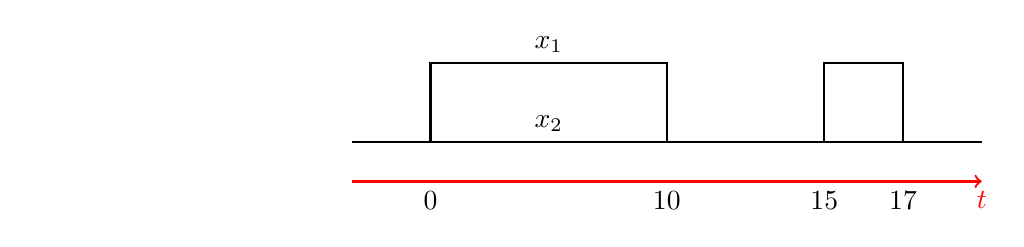
\begin{tikzpicture}[thick]
\centering
%%Location
\draw (-4,0) node {};
%%axis
\draw[->][red] (0,0) -- (8,0) coordinate[label = {below:$t$}] (xmax);
%%Dendrogram
\draw plot (1,0.5)--(1,1.5)--(4,1.5)--(4,0.5);

\draw plot (6,0.5)--(6,1.5)--(7,1.5)--(7,0.5);
\draw plot (0,0.5)--(8,0.5);


%%Label
\draw (1,0) node [anchor=north] {0};
\draw (4,0) node [anchor=north] {10};
\draw (6,0) node [anchor=north] {15};
\draw (7,0) node [anchor=north] {17};
\draw (2.5,1.5) node [anchor=south] {$x_1$};
\draw (2.5,0.5) node [anchor=south] {$x_2$};

\end{tikzpicture}
\caption{Formigram $\theta_X$}
\end{figure}
\begin{figure}[h]
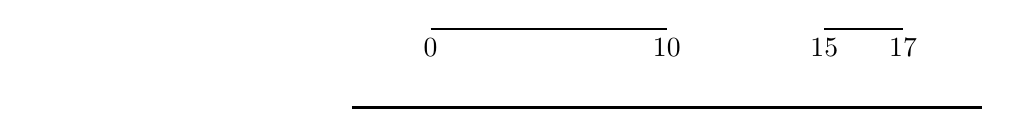
\begin{tikzpicture}[thick]
\centering
%%Location
\draw (-4,0) node {};
%%Dendrogram
\draw plot (1,0.5)--(4,0.5);

\draw plot (6,0.5)--(7,0.5);
\draw plot (0,-0.5)--(8,-0.5);


%%Label
\draw (1,0.5) node [anchor=north] {0};
\draw (4,0.5) node [anchor=north] {10};
\draw (6,0.5) node [anchor=north] {15};
\draw (7,0.5) node [anchor=north] {17};
\end{tikzpicture}
\caption{$\dgm(\mathcal{X})$}
\end{figure}

Observe the following.
\begin{itemize}
\item $\mathbf{t}_{\mathcal{X}}(x_1)=[0,10)\cup[15,17)$ and $\mathbf{t}_{\mathcal{X}}(x_2)=(-\infty, \infty)$
\item $t_{\theta_X}(x_1,x_2)=(-\infty,0)\cup(10,15]\cup(17,\infty)=\mathbb{R}\setminus \mathbf{t}_{\mathcal{X}}(x_1)$
\item $\dgm(\mathcal{X})=\{[0,10), [15,17),(-\infty,\infty)\}$
\end{itemize}
\end{example}

 
\newpage

\begin{example}  

Consider an ordered formigram $\mathcal{X}=(X, \theta_X, \mathfrak{o}_X)$ defined as below where $(X,\mathfrak{o}_X)=\{x_1<x_2<x_3\}$.



\begin{figure}[h]
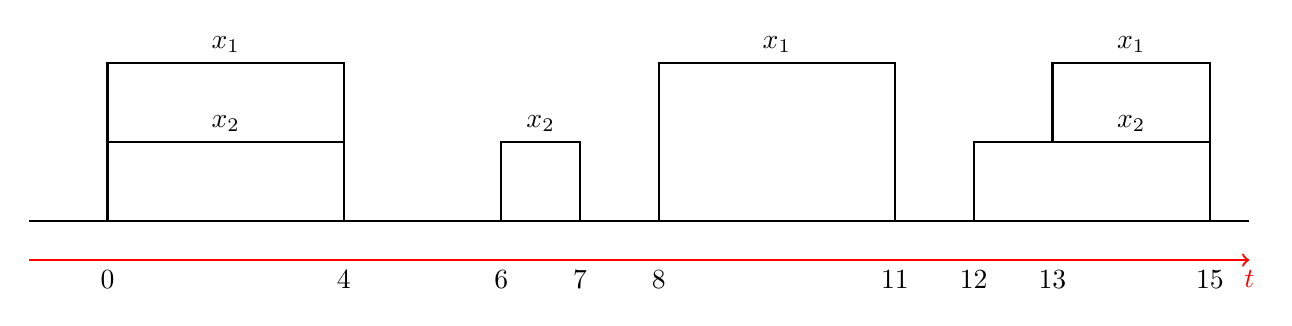
\begin{tikzpicture}[thick]
\centering
%%axis
\draw[->][red] (0,0) -- (15.5,0) coordinate[label = {below:$t$}] (xmax);
%%Dendrogram
\draw plot (1,0.5)--(1,1.5)--(4,1.5)--(4,0.5);
\draw plot (1,1.5)--(1,2.5)--(4,2.5)--(4,1.5);
\draw plot (8,0.5)--(8,2.5)--(11,2.5)--(11,0.5);
\draw plot (12,0.5)--(12,1.5)--(15,1.5)--(15,0.5);
\draw plot (13,1.5)--(13,2.5)--(15,2.5)--(15,1.5);
\draw plot (6,0.5)--(6,1.5)--(7,1.5)--(7,0.5);
\draw plot (0,0.5)--(15.5,0.5);

%%Label
\draw (1,0) node [anchor=north] {0};
\draw (4,0) node [anchor=north] {4};
\draw (6,0) node [anchor=north] {6};
\draw (7,0) node [anchor=north] {7};
\draw (8,0) node [anchor=north] {8};
\draw (11,0) node [anchor=north] {11};
\draw (12,0) node [anchor=north] {12};
\draw (13,0) node [anchor=north] {13};
\draw (15,0) node [anchor=north] {15};
\draw (2.5,2.5) node [anchor=south] {$x_1$};
\draw (2.5,1.5) node [anchor=south] {$x_2$};
\draw (6.5,1.5) node [anchor=south] {$x_2$};
\draw (9.5,2.5) node [anchor=south] {$x_1$};
\draw (14,1.5) node [anchor=south] {$x_2$};
\draw (14, 2.5) node [anchor=south] {$x_1$};
\end{tikzpicture}
\caption{Formigram $\theta_X$}
\end{figure}
\begin{figure}[h]\label{fig8}
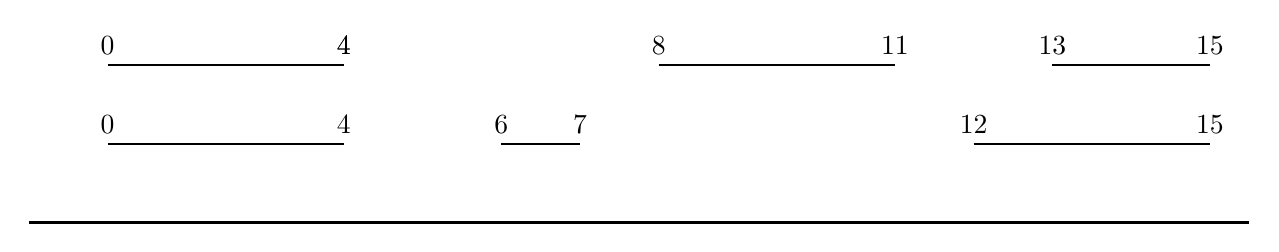
\begin{tikzpicture}[thick]
\centering
%%Dendrogram
\draw plot (1,1.5)--(4,1.5);
\draw plot (1,2.5)--(4,2.5);
\draw plot (8,2.5)--(11,2.5);
\draw plot (12,1.5)--(15,1.5);
\draw plot (13,2.5)--(15,2.5);
\draw plot (6,1.5)--(7,1.5);
\draw plot (0,0.5)--(15.5,0.5);

%%Label
\draw (4,2.5) node [anchor=south] {4};
\draw (1,2.5) node [anchor=south] {0};
\draw (4,1.5) node [anchor=south] {4};
\draw (1,1.5) node [anchor=south] {0};
\draw (6,1.5) node [anchor=south] {6};
\draw (7,1.5) node [anchor=south] {7};
\draw (4,2.5) node [anchor=south] {4};
\draw (8,2.5) node [anchor=south] {8};
\draw (11,2.5) node [anchor=south] {11};
\draw (12,1.5) node [anchor=south] {12};
\draw (15,1.5) node [anchor=south] {15};
\draw (15,2.5) node [anchor=south] {15};
\draw (13,2.5) node [anchor=south] {13};
\end{tikzpicture}
\caption{$\dgm(\mathcal{X})$}
\end{figure}
\begin{itemize}
\item $\mathbf{t}_{\mathcal{X}}(x_1)=[0,4)\cup[8,11)\cup [13,15)$, $\mathbf{t}_{\mathcal{X}}(x_2)=[0,4)\cup[6,7)\cup [12,15)$ and $\mathbf{t}_{\mathcal{X}}(x_3)=(-\infty, \infty)$
\item $\dgm(\mathcal{X})=\{[0,4), [0,4), [6,7), [8,11), [12,15), [13,15),(-\infty,\infty)\}$

\item $\mathbf{t}_{\mathcal{X}}(x_i)$ consists of the bars at the $i$-th row in Figure 6 for each $i=1,2,3$.
\end{itemize}

\end{example}

\subsection{The Relationship Between The Set-Theoretical Persistent Diagrams and Original Persistent Diagrams.} 

\subsubsection{Case of Dendrograms}

 After showing a lemma below, we are going to prove that the set-theoretic persistent diagram is identical to the persistent diagram derived from linearization in the case of dendrograms.
\begin{lemma} Let $(X,\theta_X, \mathfrak{o}_X)$ be an ordered dendrogram. Then $$\{t(x):x \in X\}\setminus \{\infty\}=\mathrm{Spec}(\mathcal{U}_{\theta_X})\setminus \{0\}$$ as a set where $t(x)$ is defined in Definition \ref{defeat2}.

\begin{proof}
Take $x\in X$ which is not the maximum in the order $<$ so that $t(x)<\infty$.  There exists $x'\in X$ such that $x'\in [x]_{t(x)}$ and $x<x'$. Then $\mathcal{U}_{\theta_X}(x,x')=t(x)$ because $x'$ cannot be in the same block with $x$ before the time $t(x)$ by the definition of $t(x)$. Therefore, $t(x)\in \mathrm{Spec}(\mathcal{U}_{\theta_X})$.\par 
On the other hand, take $u_i\in \mathrm{Spec}(\mathcal{U}_{\theta_X})\setminus \{0\}=\{u_1< u_2<\cdots< u_m\}$. Then there are $x_1,x_2\in X$ such that $u_i=\mathcal{U}_{\theta_X}(x_1,x_2)$. Note that $[x_1]_{u_{i-1}}\neq [x_2]_{u_{i-1}}$ since the blocks containing $x_1$ and $x_2$ merge at the time $u_i$. Let $x=\max[x_1]_{u_{i-1}}$ and $x'=\max[x_2]_{u_{i-1}}$. Without loss of generality, we may assume $x<x'$. This implies $u_i=t(x)$.\end{proof}

\end{lemma}

\begin{proposition} Let $(X,\theta_X, \mathfrak{o}_X)$ be an ordered dendrogram so that $t:X\rightarrow [0,\infty]$ is defined as Definition \ref{defeat2}
Then, as a multiset:
$$\dgm(\theta_X)=\dgm(\mathcal{X})$$
\begin{proof}
 We already know an easy way to compute $\dgm(\theta_X)$ by proposition \ref{dgm2} and $\dgm(\mathcal{X})=\{[0,t(x)): x\in X\}$ as a multiset. In order to compare the two multisets $\dgm(\mathcal{X})$ and $\dgm(\theta_X)$, we use the notation $\#_1$ to denote the multiplicity of elements in $\dgm(\mathcal{X})$ and use $\#_2$ for elements in $\dgm(\theta_X)$. By the previous lemma, $\{t(x):x \in X\}\setminus \{\infty\}=\mathrm{Spec}(\mathcal{U}_{\theta_X})\setminus \{0\}=\{u_1< u_2<\cdots, u_n\}$ as a set. Let $x\in X$ be a non-maximal element and consider $t(x)=u_i\in \mathrm{Spec}(\mathcal{U}_{\theta_X})\setminus \{0\}$. Note that $\#_1[0,t(x))$ is equal to the number of elements in $X$ which lose in the competition at $t=t(x)$. Also, this number is equal to the number of survivors at the time right before $t(x)$ minus the number of survivors at the time $t(x)$, which can be expressed in $\abs{X_{t(x)-\epsilon}}-\abs{X_{t(x)}}$ for small enough $\epsilon>0$. Now, 
\begin{align*}
\abs{X_{t(x)-\epsilon}}-\abs{X_{t(x)}}&=\abs{X_{u_i-\epsilon}}-\abs{X_{u_i}}&&\because t(x)=u_i\\&=\abs{X_{u_{i-1}}}-\abs{X_{u_i}}&&\because \epsilon \ \mbox{is small enough}\\&=\abs{\theta_X(u_{i-1})}-\abs{\theta_X(u_i)}&&\mbox{By Remark}\ \ref{num}\\&=\#_2[0,u_i) &&\mbox{By Proposition \ref{dgm2}}
\end{align*}
Therefore, we have $\#_1[0,t(x))=\#_2[0,t(x))$ for all $x\in X$ but the maximum of $X$. But, the fact that both $\dgm(\mathcal{X})$ and $\dgm({\theta_X})$ contains one $[0,\infty)$ finishes the proof.\end{proof}\label{dgm3}
\end{proposition}

\begin{remark}Note that we chose an arbitrary order on $X$ in the above proof.
\end{remark}

\subsubsection{Case of Formigrams}

\begin{example} Let $\mathcal{X}=(X,\theta_X, \mathfrak{o}_X)$ and $\mathcal{X}'=(X,\theta_X,\mathfrak{o}_X' )$ be formigrams such that $(X,\mathfrak{o}_X)=\{x_1<x_2<x_3\}$ and $(X,\mathfrak{o}_X')=\{x_2<x_3<x_1\}$ and $\theta_X$ on $X$ is given below. 
\begin{figure}[h]
\begin{tikzpicture}[thick]
\centering
%%Location
\draw (-4,0) node {};
%%axis
\draw[->][red] (-1,0) -- (9,0) coordinate[label = {below:$t$}] (xmax);
%%Dendrogram
\draw plot (1,0.5)--(1,1.5)--(4,1.5)--(4,0.5);
\draw plot (2,1.5)--(2,2.5)--(7,2.5)--(7,1.5);

\draw plot (6,0.5)--(6,1.5)--(7,1.5)--(7,0.5);
\draw plot (-1,0.5)--(9,0.5);


%%Label
\draw (1,0) node [anchor=north] {0};
\draw (2,0) node [anchor=north] {3};
\draw (4,0) node [anchor=north] {10};
\draw (6,0) node [anchor=north] {15};
\draw (7,0) node [anchor=north] {17};
\draw (5,2.5) node [anchor=south] {$x_1$};
\draw (3.5,1.5) node [anchor=south] {$x_2$};
\draw (3.5,0.5) node [anchor=south] {$x_3$};
\draw (6.5,1.5) node [anchor=south] {$x_2$};

\end{tikzpicture}
\caption{Formigram $\theta_X$}
\end{figure}\label{ex3}
\end{example}

We can see that two ordered formigrams whose only difference is the order on the underlying set have different set-theoretical persistent diagrams as Figure 8 and 9.

\begin{figure}[h]
\begin{tikzpicture}[thick]
\centering
%%Location
\draw (-4,0) node {};
%%Dendrogram
\draw plot (1,1.5)--(4,1.5);
\draw plot (2,2.5)--(7,2.5);

\draw plot (6,1.5)--(7,1.5);
\draw plot (-1,0.5)--(9,0.5);


%%Label
\draw (1,1.5) node [anchor=north] {0};
\draw (4,1.5) node [anchor=north] {10};
\draw (6,1.5) node [anchor=north] {15};
\draw (7,1.5) node [anchor=north] {17};
\draw (2,2.5) node [anchor=north] {3};
\draw (7,2.5) node [anchor=north] {17};
\draw (-1,0.5) node [anchor=north] {$-\infty$};
\draw (9,0.5) node [anchor=north] {$\infty$};
\end{tikzpicture}
\caption{${\dgm}(\mathcal{X})$ with the order $x_1<x_2<x_3$}
\end{figure}

\medskip

\begin{figure}[h]
\begin{tikzpicture}[thick]
\centering
%%Location
\draw (-4,0) node {};
%%Dendrogram
\draw plot (1,1.5)--(7,1.5);
\draw plot (2,2.5)--(4,2.5);
\draw plot (6,2.5)--(7,2.5);


\draw plot (-1,0.5)--(9,0.5);
%%Label
\draw (1,1.5) node [anchor=north] {0};
\draw (4,2.5) node [anchor=north] {10};
\draw (6,2.5) node [anchor=north] {15};
\draw (7,1.5) node [anchor=north] {17};
\draw (2,2.5) node [anchor=north] {3};
\draw (7,2.5) node [anchor=north] {17};
\draw (-1,0.5) node [anchor=north] {$-\infty$};
\draw (9,0.5) node [anchor=north] {$\infty$};
\end{tikzpicture}
\caption{$\dgm(\mathcal{X}')$ with the order $x_2<x_3<x_1$}
\end{figure}

However, two diagrams share the following property: For each $t\in \mathbb{R}$, the number of intervals including $t$ in $\dgm(\mathcal{X})$ is equal to the number of ones in $\dgm(\mathcal{X}')$.
\newpage

\section{Stability Results for Dendrograms}

The following proposition indicates the ordering on $X$ can be helpful to prove the stability between $\mathrm{dist}(\theta_X,\theta_Y)$ and $d_B(\dgm(\theta_X), \dgm(\theta_Y))$


\begin{proposition} Fix $\eta>0$. Let $\mathcal{U}$ and $\mathcal{U}'$ be two ultrametrics on $X$ induced by dendrograms $\theta_X$ and $\theta'_X$ respectively satisfying $\norm{\mathcal{U}-\mathcal{U'}}_{\infty}\leq \eta.$ Then, there exists a bijection $\varphi:\dgm(\theta_X)\rightarrow \dgm(\theta'_X)$ such that $\norm{I-\varphi(I)}_{\infty}\leq \eta$ for all $I\in \dgm(\theta_X)$. Therefore, we also have $d_B(\dgm(\theta_X), \dgm(\theta_X'))\leq \eta$.

\begin{proof}
We shall construct a bijection $\varphi:\dgm(\theta_X)\rightarrow \dgm(\theta'_X)$ such that $\norm{I-\varphi(I)}_{\infty}\leq \eta$ for all $I\in \dgm(\theta_X)$. As a strategy, assign an arbitrary total order $<$ on $X$, which allows us to have succinct representation for $\dgm(\theta_X)$ and $\dgm(\theta'_X)$. Recall that once we assign an order on $X$, the functions $t, t':X\rightarrow [0,\infty]$ are naturally defined for dendrograms $\theta_X$ and $\theta'_X$ respectively as Definition \ref{defeat2}. Furthermore, we are equipped with the following representation for persistent diagrams by Proposition \ref{dgm3}. 
\begin{align*}
\dgm(\theta_X)=\{[0,t(x)): x\in X\}\\
\dgm(\theta_X')=\{[0,t'(x)): x\in X\}
\end{align*}
Now, define $\varphi:\dgm(\theta_X)\rightarrow \dgm(\theta'_X)$ by $[0,t(x))\mapsto [0,t'(x))$ and we shall show that $\norm{[0,t(x))-[0,t'(x))}_{\infty}=\abs{t(x)-t'(x)}\leq \eta$ for every non-maximal $x\in X$.\footnote{For $x=\max X$, $[0,t(x))=[0,t'(x))=[0,\infty)$.} Take $x\in X$ which is not maximal of $X$. Then $t(x)<\infty$, and there exists $y>x$ such that $y\in [x]_{t(x)}^{\mathcal{U}}$. Note that $\mathcal{U}'(x,y)\leq t(x)+\eta$ because $\mathcal{U}'(x,y)\leq \mathcal{U}(x,y)+\eta$ and $\mathcal{U}(x,y)\leq t(x)$. Therefore, $y\in[x]_{t(x)+\eta}^{\mathcal{U}'}$ and $t'(x)\leq t(x)+\eta$. By symmetry, $t(x)\leq t'(x)+\eta$ as well and hence $\abs{t(x)-t'(x)}\leq \eta$ as desired.\end{proof} \label{prop4.7}
\end{proposition}
The next proposition is nothing but another definition of Gromov-Hausdorff distance.


\begin{proposition} Consider two metric spaces $(X, d_X)$ and $(Y,d_Y)$. Let $Z$ be a set and $f_X:Z\rightarrow X$ and $f_Y:Z\rightarrow Y$ be surjective maps. Then 
$$d_{GH}(X,Y)\leq \frac{1}{2}\norm{f^*_Xd_X-f^*_Yd_Y}_{\infty}$$
In fact, $\displaystyle d_{GH}(X,Y)=\frac{1}{2}\inf_{Z,f_X,f_Y}\norm{f^*_Xd_X-f^*_Yd_Y}_{\infty}$\label{prop4.8}
\end{proposition}

\begin{proposition}For any two dendrograms $\theta_X, \theta_Y$ on $X$ and $Y$ respectively,

$$2 \,\mathrm{dist}(\theta_X, \theta_Y)\geq d_B(\dgm(\theta_X), \dgm(\theta_Y))$$

\begin{proof} 
Assume that $\eta>d_{GH}((X,\mathcal{U}_{\theta_X}),(Y, \mathcal{U}_{\theta_Y}))$ for some $\eta>0$. By proposition \ref{prop4.8}, there exist a set $Z$ and surjections $f_X:Z\rightarrow X$, $f_Y:Z\rightarrow Y$ such that $2\eta> \norm{\mathcal{U}-\mathcal{U'}}_{\infty}$ where $\mathcal{U}=f^*_X\mathcal{U}_{\theta_X}$ and $\mathcal{U}'=f^*_Y\mathcal{U}_{\theta_Y}$. By Proposition \ref{prop4.7}, we have %Assign an order $<$ on $Z$ arbitrarily. %satisfying the following property:
%$$f_X(z_1)<f_X(z_2) \Rightarrow z_1<' z_2$$
%Now, we can define the function $t:Z\rightarrow \mathbb{R}^+$ as the definition \ref{defeat} and
$$\displaystyle d_B(\dgm(\mathcal{U}), \dgm(\mathcal{U}'))\leq 2\eta.$$ On the other hand, applying triangle inequality for the bottleneck distance,
\begin{align*}
d_B(\dgm(\theta_X),\dgm(\theta_Y))&\leq d_B(\dgm(\theta_X), \dgm(\mathcal{U}))+d_B(\dgm(\mathcal{U}),\dgm(\mathcal{U}'))+d_B(\dgm(\mathcal{U}'), \dgm(\theta_Y))\\&\leq d_B(\dgm(\theta_X), \dgm(\mathcal{U}))+d_B(\dgm(\mathcal{U}'), \dgm(\theta_Y))+2\eta
\end{align*}
But, it will be proven that $d_B(\dgm(\theta_X), \dgm(\mathcal{U}))=d_B(\dgm(\mathcal{U}'),\dgm(\theta_Y))=0$ in the following lemma and thus 
$$d_B(\dgm(\theta_X), \dgm(\theta_Y))\leq 2\eta.$$ Since $\eta$ was arbitrarily chosen, we obtain the desired result. \label{stability2}
\end{proof}
\end{proposition}
\begin{lemma} Let $(X,\mathcal{U}_{\theta_X})$ be an ultrametric space and a map $f:Z\rightarrow X$ is surjective. Then $$d_B(\dgm(\theta_X), \dgm(f^*\mathcal{U}_{\theta_X}))=0$$
\begin{proof}

Notice that $\dgm(f^*\mathcal{U}_{\theta_X})$ is nothing but $\dgm(\theta_X)\cup O$ where $O$ is the multiset consisting of a finite number of copies of $(0,0)\in \mathbb{R}^2$ only. \end{proof}
\end{lemma}

\woojin{To be precise, the pseudo-ultrametric $f^*\mathcal{U}_{\theta_X}$ does not induce a dendrogram on $Z$ because many elements can belong to a block at the beginning when inducing dendrogram-like structure from a pseudo-ultrametric. In my opinion, $\dgm(f^*\mathcal{U}_{\theta_X})$ should be just defined as the persistent diagram of quotient space $Z/f^*\mathcal{U}_{\theta_X}$, which is exactly the same as $\dgm(\theta_X)$.}





\section{Stability Results for Formigrams}

We approach to stability theorem in two ways: one way is relevant to order on the underlying set whereas another is purely related to linearization.

\subsection{Stability results for set-theoretic persistent diagrams.}

\subsubsection{Groundwork}

First, we introduce some terms we are going to use frequently.
\begin{definition}
To say that $\mathcal{A}$ is an intervals' system means that 
\begin{itemize}
\item $\mathcal{A}$ is a non-empty finite collection of half-open intervals of the form $[a,b)$ in $\mathbb{R}\cup \{-\infty\}$ allowing $a$ to be $-\infty$. 

\item Not only any two distinct elements in $\mathcal{A}$ are disjoint but also they do not share their endpoints.
\end{itemize}
\end{definition}


\begin{definition} Let $\mathcal{A}=\{I_i=[a_i,b_i):  1\leq i \leq m\}$ be an intervals' system. \label{interval}

\begin{itemize}
\item (The set of endpoints) $E_\mathcal{A}:= \{a_i, b_i: 1\leq i \leq m\}\subset \mathbb{R}\cup \{-\infty\}$

\item (Complement of system) Letting $b_0=-\infty$ and $a_{m+1}=\infty$ as definition,  $\displaystyle C(\mathcal{A}):=\mathbb{R}\setminus \cup \mathcal{A}=\dotcup_{i=0}^m[b_i,a_{i+1})$ 
\end{itemize}
\end{definition}
Observe that $\abs{E_\mathcal{A}}=2m$ since  any two intervals in $\mathcal{A}$ do not share their endpoints. 

\begin{theorem}\label{stability}
Given two intervals' systems $\mathcal{A}=\{I_i=[a_i,b_i):  1\leq i \leq m\}$ and $\mathcal{B}=\{J_j=[c_j,d_j): 1\leq j \leq n\}$ 
\begin{align*}
d_{H}^\mathbb{R}\big(C(\mathcal{A}) ,C(\mathcal{B})\big)= d_B(\mathcal{A}, \mathcal{B})
\end{align*}
where $d_B(\mathcal{A}, \mathcal{B})=\min\{\delta\geq 0|\,\exists \sigma\,\,\mbox{a $\delta$-matching between $\mathcal{A}$ and $\mathcal{B}$}\}$.
\end{theorem}

%\woojin{Before I left Columbus, we were mainly working on the proof for $d_{H}^\mathbb{R}\big(C(\mathcal{A}) ,C(\mathcal{B})\big)\geq d_B(\mathcal{A}, \mathcal{B})$ and we thought we succeeded to prove it in the case of $\abs{\mathcal{B}}=1$ by induction on $\abs{\mathcal{A}}$ However, I've realized that our proof was incomplete. You will see the trouble in the proof below.}
%\facundo{Why do you need that induction argument? i thought we had circumvented that line of argument?} \woojin{Yes, ignore this comment.}\facundo{ok}.


First, we are going to prove $d_{H}^\mathbb{R}\big(C(\mathcal{A}) ,C(\mathcal{B})\big)\leq d_B(\mathcal{A}, \mathcal{B})$  after showing a lemma. 

\begin{lemma} $\displaystyle d_H^\mathbb{R}(C(\mathcal{A}), C(\mathcal{B}))=\max\{\max_{a\in C(\mathcal{A})\cap (\cup \mathcal{B})}\min_{b\in E_\mathcal{B}} \abs{a-b}, \max_{b\in C(\mathcal{B})\cap (\cup \mathcal{A})}\min_{a\in E_\mathcal{A}}\abs{a-b}\}$
\begin{proof} Recalling that 
$$d_H^\mathbb{R}(C(\mathcal{A}), C(\mathcal{B}))=\max\{\max_{a\in C(\mathcal{A})}\min_{b\in C(\mathcal{B})}\abs{a-b}, \max_{b\in C(\mathcal{B})}\min_{a\in C(\mathcal{A})}\abs{a-b}\},$$
it suffices to prove only that
\begin{equation}\label{max}
\max_{a\in C(\mathcal{A})}\min_{b\in C(\mathcal{B})}\abs{a-b}=\max_{a\in C(\mathcal{A})\cap (\cup \mathcal{B})}\min_{b\in E_\mathcal{B}} \abs{a-b}
\end{equation}
by symmetry. Let $\displaystyle \varphi(a):=\min_{b\in C(\mathcal{B})}\abs{a-b}$ for all $a\in C(\mathcal{A})$. Then $\varphi(a)=0$ if $a\in C(\mathcal{B})$ evidently and hence restricting the domain $C(\mathcal{A})$ of $\varphi$ to the intersection of $C(\mathcal{A})$ and $\mathbb{R}\setminus C(\mathcal{B})=\cup \mathcal{B}$ does not affect the maximum of $\varphi$, which means
\begin{equation}\label{max1}
\max_{a\in C(\mathcal{A})}\min_{b\in C(\mathcal{B})}\abs{a-b}=\max_{a\in C(\mathcal{A})\cap (\cup\mathcal{B})}\min_{b\in C(\mathcal{B})}\abs{a-b}.
\end{equation}
Next, fix an arbitrary $a\in \cup \mathcal{B}$. Then the closest point in $\mathbb{R}\setminus \cup \mathcal{B}=C(\mathcal{B})$ to $a$ is obviously located on the boundary of $C(\mathcal{B})$, the set of endpoints $E_\mathcal{B}$, which implies 

\begin{equation*}
\min_{b\in C(\mathcal{B})}\abs{a-b}=\min_{b\in E_{\mathcal{B}}}\abs{a-b}
\end{equation*}
for arbitrary $a\in \cup \mathcal{B}$.

Therefore, we have
\begin{equation}\label{max2}
\max_{a\in C(\mathcal{A})\cap (\cup\mathcal{B})}\min_{b\in C(\mathcal{B})}\abs{a-b}=\max_{a\in C(\mathcal{A})\cap (\cup \mathcal{B})}\min_{b\in E_\mathcal{B}} \abs{a-b}
\end{equation}
Equations (\ref{max1}) and (\ref{max2}), yield the desired result (\ref{max}). 
\end{proof}
\end{lemma}

\textbf{The proof for $d_{H}^\mathbb{R}\big(C(\mathcal{A}) ,C(\mathcal{B})\big)\leq d_B(\mathcal{A}, \mathcal{B})$.}\\ 

Let $\sigma:\mathcal{A} \nrightarrow \mathcal{B}$
be a $\delta$-matching. By the previous lemma and symmetry, it suffices to prove that $$\max_{a\in C(\mathcal{A})\cap (\cup \mathcal{B})}\min_{b\in E_\mathcal{B}} \abs{a-b}\leq \delta.$$

Fix an $a\in C(\mathcal{A})\cap (\cup \mathcal{B})$. Then there are $0\leq i\leq m$ and $1\leq j \leq n$ such that 

\begin{equation}\label{intersection}
a\in [b_i, a_{i+1})\cap [c_j,d_j) 
\end{equation}

\textbf{Case 1.} Assume that length$(c_j,d_j]\leq 2\delta$. Then 
\begin{align*}
\min_{b\in E_{\mathcal{B}}}\abs{a-b}&\leq \min \{\abs{a-c_j}, \abs{a-d_j}\}\leq \delta 
\end{align*}

because $a\in [c_j, d_j)$ and the length of $[c_j,d_j)$ is $\leq 2\delta$.

\vspace{3mm}

\textbf{Case 2.} Assume that length$(c_j,d_j]>2\delta$. Then there exists $1\leq k\leq m$ such that $(a_k, b_k]$ is matched with $(c_j,d_j]$ via $\sigma$ because $\sigma$ is a $\delta$-matching. Note that the intersection of two intervals in (\ref{intersection}) can be possibly expressed as follows:

$$[b_i, a_{i+1})\cap [c_j,d_j)=\begin{cases} [c_j,d_j)& \mbox{Case (a)} \\ [b_i, a_{i+1})& \mbox{Case (b)}\\ [b_i, d_j)& \mbox{Case (c)} \\ [c_j, a_{i+1})& \mbox{Case (d)} \end{cases} $$

Assume that Case (a) happens, which implies $J_j=[c_j,d_j)\subset [b_i,a_{i+1})$ (See Figure below). In this case, it is easy to see that the closest intervals to $[c_j, d_j)$ in $\mathcal{A}$ in the metric  $\norm{\cdot}_\infty$ are $[a_i, b_i)$ and $[a_{i+1}, b_{i+1})$. However, both $\norm{I_i-J_j}_\infty$ and $\norm{I_{i+1}- J_j}_\infty$ are greater than $\delta$ because $2\delta \leq \abs{b_i-d_j} \leq \norm{I_i-J_j}_\infty$ and $2\delta \leq \abs{a_{i+1}-c_j} \leq \norm{I_{i+1}- J_j}_\infty$. This contradicts the fact that $\sigma$ is a $\delta$-matching. Therefore, Case (a) cannot happen. \par

Next, assume Case (b). Also, assume that $[c_j,d_j)$ is matched with $I_k$ for $k\leq i$ via $\sigma$. Then since $b_k\leq b_i\leq a \leq d_j$ and $\abs{b_k-d_j}\leq \delta$, we also have $\abs{a-d_j}\leq \delta$. Now, suppose that  $[c_j,d_j)$ is matched with $I_k$ for $k> i$. Then one can show that $\abs{a-c_j}\leq \delta$ in the same way. In each case, $\displaystyle \min_{b\in E_{\mathcal{B}}}\abs{a-b}\leq \min\{\abs{a-c_j}, \abs{a-d_j}\} \leq \delta$ as desired. \par

Suppose Case (c) occurs, i.e., $c_j \leq b_i \leq d_j \leq a_{i+1}$. Note that $I_k$ cannot be matched with $J_j$ for $k>i$ via $\sigma$ because $c_j<d_j\leq a_{i+1}$ and $\delta< 2\delta < d_j-c_j \leq a_{i+1}-c_j \leq a_k-c_j \leq \norm{I_k-J_j}_{\infty}$. Hence, $J_j$ must be matched with $I_k$ for $k\leq i$.  This implies that $b_k<b_i\leq a < d_j$ and $d_j-b_k\leq \norm{J_j-I_k}_\infty<\delta$ and in turn $\abs{a-d_j}<\delta.$  In Case (d), one can check that $\abs{a-c_j}<\delta$ in the same way as well. We have shown that $\displaystyle \min_{b\in E_{\mathcal{B}}}\abs{a-b}\leq \delta$ for all $a\in C(\mathcal{A})\cap (\cup \mathcal{B})$ as desired. One can also prove $\displaystyle \max_{b\in C(\mathcal{B})\cap (\cup \mathcal{A})}\min_{a\in E_\mathcal{A}}\abs{a-b}\leq \delta$ in the same way.\endproof

\begin{figure}[b] 
\begin{tikzpicture}
\centering
%%Location
\draw (-6,0) node {};

\draw plot (-3,1.5)--(-0.5,1.5);
\draw plot (6,1.5)--(8,1.5);
\draw plot (0,0.5)--(5,0.5);

\draw (6,1.5) node [anchor=south] {$a_{i+1}$};
\draw (8,1.5) node [anchor=south] {$b_{i+1}$};

\draw (-3,1.5) node [anchor=south] {$a_{i}$};

\draw (-0.5,1.5) node [anchor=south] {$b_{i}$};
\draw (0,0.5) node [anchor=south] {$c_{j}$};
\draw (5,0.5) node [anchor=south] {$d_{j}$};

\end{tikzpicture}
\caption{This picture illustrates Case 2, (a). Two upper segments stand for $I_i$ and $I_{i+1}$ in $\mathcal{A}$ and the lower one is $J_j$ in $\mathcal{B}$.}
\end{figure}

\vspace{5mm}

\textbf{The proof for $d_{H}^\mathbb{R}\big(C(\mathcal{A}) ,C(\mathcal{B})\big)\geq d_B(\mathcal{A}, \mathcal{B})$.}\\

\vspace{3mm}

Before proceeding, we introduce some notation.
\begin{definition} Let $\mathcal{A}$ be an intervals' system and $\epsilon \geq 0$. Define $\mathcal{A}^{\epsilon}$ to be the collection of intervals in $\mathcal{A}$ of length $\geq \epsilon$.
\end{definition}

\begin{definition} Let $I=[a,b)$ be an interval and $\epsilon \geq 0$. 
$$I^{-\epsilon}:=\begin{cases} \emptyset & \mbox{if\ $\length{I}\leq 2\epsilon$}\\ [a+\epsilon, b-\epsilon ) & \mbox{otherwise} \end{cases}$$

\end{definition}

\begin{lemma} Let $\mathcal{A}=\{I_i=[a_i,b_i):  1\leq i \leq m\}$ be an intervals' system. Then, $\displaystyle \mathbb{R}\setminus \big(C(\mathcal{A})\big)^\eta=\bigcup_{I\in A^{2\eta}} I^{-\eta}$

\begin{proof}
It is easy to check the equality holds when $\mathcal{A}$ consists of only one interval. In general, $C(\mathcal{A})=\mathbb{R}\setminus \cup \mathcal{A}=\mathbb{R} \setminus \bigcup_{i=1}^m I_i$ as Definition \ref{interval} and

\begin{align*}
\mathbb{R}\setminus \big(C(\mathcal{A})\big)^\eta&=\mathbb{R}\setminus\big(\mathbb{R} \setminus \bigcup_{i=1}^m I_i \big)^\eta 
\\&=\mathbb{R}\setminus \big(\bigcap_{i=1}^m(\mathbb{R} \setminus I_i)\big)^\eta
\\&\stackrel{(*)}{=}\mathbb{R}\setminus \big(\bigcap_{i=1}^m(\mathbb{R}\setminus I_i)^\eta \big)&\mbox{Proved below}
\\&= \bigcup_{i=1}^m\big(\mathbb{R}\setminus (\mathbb{R}\setminus I_i)^\eta\big)
\\&=\bigcup_{I_i \in \mathcal{A}^{2\eta}} (I_i)^{-\eta}
\end{align*}
In order to justify that the equality with  (*) holds, we shall prove that $$\big(\bigcap_{i=1}^m(\mathbb{R} \setminus I_i)\big)^\eta=\bigcap_{i=1}^m(\mathbb{R}\setminus I_i)^\eta.$$
Since $\bigcap_{i=1}^m(\mathbb{R} \setminus I_i)\subset \mathbb{R}\setminus I_j$ for all $1\leq j \leq m$, $\big(\bigcap_{i \in A}(\mathbb{R} \setminus I_i)\big)^\eta \subset (\mathbb{R}\setminus I_j)^\eta$ for all $1\leq j \leq m$ and hence $\big(\bigcap_{i=1}^m(\mathbb{R} \setminus I_i)\big)^\eta\subset \bigcap_{i=1}^m(\mathbb{R}\setminus I_i)^\eta$. Now, take an element $x\in \bigcap_{i=1}^m(\mathbb{R}\setminus I_\alpha)^\eta$. If $x\in \bigcap_{i=1}^m(\mathbb{R}\setminus I_i)$, then obviously, $x\in \big(\bigcap_{i=1}^m(\mathbb{R} \setminus I_i)\big)^\eta$.
But, if $x\notin \bigcap_{i=1}^m(\mathbb{R}\setminus I_i)$, then there exists $1\leq i\leq m$ such that $x\notin \mathbb{R}\setminus I_i$ whereas $x\in (\mathbb{R}\setminus I_i)^\eta$. Denoting $I_i=[a,b)$, this means that $x\in [a, a+\eta)$ or $x\in (b-\eta,b)$. Whatever the case is, one can find  $\epsilon>0$ and $y\in \mathbb{R}$ such that $y\in (a-\epsilon, a)\cup [b,b+\epsilon) \subset \bigcap_{i=1}^m(\mathbb{R} \setminus I_i)$ and $\abs{x-y}<\eta$. Therefore, $\bigcap_{i=1}^m(\mathbb{R}\setminus I_i)^\eta \subset \big(\bigcap_{i=1}^m(\mathbb{R} \setminus I_i)\big)^\eta$ as desired.
\end{proof}
\end{lemma}

Let $\mathcal{A}=\{I_i=[a_i,b_i):  1\leq i \leq m\}$ and $\mathcal{B}=\{J_j=[c_j,d_j): 1\leq j \leq n\}$ be intervals' systems. Suppose that $d_{H}^\mathbb{R}\big(C(\mathcal{A}) ,C(\mathcal{B})\big)\leq \eta$ for some $\eta>0$. We wish to construct an $\eta$-matching $\sigma:\mathcal{A}\nrightarrow \mathcal{B}$ in order to show  $d_{H}^\mathbb{R}\big(C(\mathcal{A}) ,C(\mathcal{B})\big)\geq d_B(\mathcal{A}, \mathcal{B})$. Note that $C(\mathcal{B})\subset \big(C(\mathcal{A})\big)^\eta$ by assumption and thus $\bigcup_{j=1}^nJ_j=\mathbb{R}\setminus C(\mathcal{B})\supset \mathbb{R}\setminus \big(C(\mathcal{A})\big)^\eta=\bigcup_{I_i\in \mathcal{A}^{2\eta}} I_i^{-\eta}$. This implies that there exists $j$ such that $I_i^{-\eta}\subset J_j$, equivalently $I_i\subset J_j^\eta$, for each $I_i\in \mathcal{A}^{2\eta}$ since the union $\bigcup_{j=1}^nJ_j$ is disjoint. We already have shown the following proposition.
\begin{proposition}
Let $\mathcal{A}=\{I_i=[a_i,b_i):  1\leq i \leq m\}$ and $\mathcal{B}=\{J_j=[c_j,d_j): 1\leq j \leq n\}$ be intervals' systems. Assume that $\eta\geq d_{H}^\mathbb{R}\big(C(\mathcal{A}),C(\mathcal{B})\big)$ for some $\eta>0$. Then, there exist functions $f:A^{2\eta}\rightarrow B$ and $g:B^{2\eta}\rightarrow A$ such that 
$$I_i \subseteq (J_{f(i)})^\eta\,\,\mbox{for all $i\in A^{2\eta}$ and } J_j \subseteq (I_{g(j)})^\eta\,\,\mbox{for all $j\in B^{2\eta}$}$$ where $A^{2\eta}=\{1\leq i \leq m: I_i\in \mathcal{A}^{2\eta}\}$ and $B^{2\eta}=\{1\leq j \leq n: J_j \in \mathcal{B}^{2\eta}\}$. 
\end{proposition}

We are going to investigate more functions $f$ and $g$ in the above proposition and eventually construct an $\eta$-matching between $\mathcal{A}$ and $\mathcal{B}$ as we wanted.
Write $A^{2\eta}=A^{2\eta}_0\dotcup A^{2\eta}_\ast$ and $B^{2\eta}=B^{2\eta}_0\dotcup B^{2\eta}_\ast$ where

$$A^{2\eta}_0:=\{i\in A^{2\eta}: f(i)\notin B^{2\eta}\},$$

$$A^{2\eta}_{*}:=\{i\in A^{2\eta}:f(i)\in B^{2\eta}\},$$

$$B_0^{2\eta}:=\{j\in B^{2\eta}:g(j)\notin A^{2\eta}\},$$

$$B^{2\eta}_\ast:=\{j\in B^{2\eta}:g(j)\in A^{2\eta}\}.$$


\begin{claim}\label{one-to-one} $g\circ f|_{A^{2\eta}_{*}}=\mathrm{id}_{A^{2\eta}_{*}}$  and $f\circ g|_{B^{2\eta}_{*}}=\mathrm{id}_{B^{2\eta}_{*}}$ 

\end{claim}
\begin{proof}
We only show the first equality. Take an $i \in A^{2\eta}_\ast$. We know that 
\begin{equation*}
I_i \subseteq \big(J_{f(i)}\big)^\eta\subseteq \bigg(\big(I_{g(f(i))}\big)^\eta\bigg)^\eta = \big(I_{g(f(i))}\big)^{2\eta}.
\end{equation*}
Let $j=g(f(i))$. The above equation means that $[a_i,b_i)\subseteq [a_j-2\eta,b_j+2\eta)$. However, this is impossible unless either $[a_i,b_i)$ and $[a_j,b_j)$ share one of their endpoints or have non-empty intersection recalling $\mathrm{length}[a_i,b_i)\geq 2\eta$. This implies $i=j$ according to the definition of intervals' system. 
\end{proof}

Notice two important implications of the above claim: The first is that $f(A_*^{2\eta})\subseteq B_*^{2\eta}$ and $g(B_*^{2\eta})\subseteq A_*^{2\eta}$. The second is that both $f|_{A^{2\eta}_{*}}$ and $g|_{B^{2\eta}_{*}}$ are injective. Now we are going to show that $f$ and $g$ are injective on $A^{2\eta}_{0}$ and $B^{2\eta}_{0}$ respectively as well.

\begin{claim}\label{injective}
The functions $f|_{A^{2\eta}_0}$ and $g|_{B^{2\eta}_0}$ are injective.
\end{claim}
\begin{proof}
We prove the claim for $f$. Assume that $i,j \in A^{2\eta}_0$, and $f(i) = f(j)=k$, which means $(J_{k})^\eta\supseteq I_i$ and $(J_{k})^\eta\supseteq I_{j}$ and hence $(J_{k})^\eta\supseteq I_i \cup I_{j}.$ Therefore,
\begin{align*}
4\eta&\geq 2\eta+\length{J_{k}}&\because i,j \in A_0^{2\eta}
\\&=\length{(J_{k})^\eta}
\\&\geq \length{I_{i}\cup I_{j}}
\end{align*}
This enforces $I_i$ and $I_j$ to have non-empty intersection since each of them has the length$\geq 2\eta$ and thus $i=j$ because $\mathcal{A}$ is an intervals' system. \end{proof}
We are now ready to define an $\eta$-matching $\sigma:\mathcal{A}\nrightarrow \mathcal{B}$. For the sake of simplicity, we would regard $\sigma$ as a matching between index sets $A$ and $B$ of $\mathcal{A}$ and $\mathcal{B}$ respectively by identifying elements in intervals' system to their indexes. 
First, define 

$$\mathrm{coim}(\sigma) = A^{2\eta}_0 \,\dotcup\, A^{2\eta}_\ast\,\dotcup \,g(B^{2\eta}_0)$$ and

$$\mathrm{im}(\sigma) = f(A^{2\eta}_0) \, \dotcup \, B^{2\eta}_\ast \,\dotcup \, B^{2\eta}_0.$$

By the definition of each component set on the RHS for both equalities, the disjointedness among them is clear. Further, notice that 
$\mathrm{coim}(\sigma)\supseteq A^{2\eta}$ and $\mathrm{im}(\sigma)\supseteq B^{2\eta}$.

Now, define $\sigma: A \nrightarrow B$ as follows:

$$\sigma(i)=\begin{cases} f(i)& \mbox{if $i\in A^{2\eta}=A^{2\eta}_*\dotcup A^{2\eta}_0$}\\ g^{-1}(i)& \mbox{if $i \in g(B_{0}^{2\eta})$}
\end{cases}$$

Especially, $\sigma$ is well-defined on $g(B_{0}^{2\eta})$ by the claim \ref{injective}. The following diagram depicts the construction of the matching:

% $$
% \begin{array}{cccccc}
% A_{2\eta}^0 & \dot\cup &  A_{2\eta}^\ast & \dot\cup & g(B_{2\eta}^0)\\
% {\bigg\downarrow}_f & & \bigg\updownarrow & & \bigg\uparrow\\
%  f(A_{2\eta}^0) & \dot\cup & B_{2\eta}^\ast & \dot\cup & B_{2\eta}^0.
% \end{array}
% $$

$$
\xymatrix{
A^{2\eta}_0 \ar[dd]_f & \dotcup &  A^{2\eta}_\ast\ar@{<->}[dd]_{f}^{g} & \dotcup & g(B^{2\eta}_0)\\
& & & & & \\
f(A^{2\eta}_0) & \dotcup & B^{2\eta}_\ast & \dotcup & B^{2\eta}_0\ar[uu]_g
}
$$

It remains to show that  $\norm{I_i-J_{\sigma(i)}}_{\infty}\leq \eta$, i.e., $I_i \subseteq (J_{\sigma(i)})^{\eta}$ and $J_{\sigma(i)}\subseteq (I_i)^{\eta}$ for all $i\in \mathrm{coim}(\sigma)$. Recall that $I_i=[a_i,b_i)$ and $J_j=[c_j,d_j)$ for $1\leq i \leq m$ and $1\leq j \leq n$. \\

\noindent\textbf{Case 1.} Pick $i\in A^{2\eta}_0$ and let $\sigma(i)=f(i)=j$ so that $\length{I_i}\geq 2\eta$ whereas $\length{J_{j}}< 2\eta$. We wish to verify that $I_i \subseteq (J_j)^{\eta}$ and $J_j\subseteq (I_i)^{\eta}$. But, the first inclusion follows automatically from the definition of $f$ and this implies that (1) $a_i\geq c_j-\eta$ and (2) $b_i\leq d_j+\eta$. So we are going to prove $J_j\subseteq (I_i)^{\eta}$ only, which amounts to show that (3) $c_j\geq a_i-\eta$ and (4) $d_j\leq b_i+\eta$. Suppose that (3) is false, i.e., $c_j<a_i-\eta$. Then we have

\begin{align*}
d_j&=c_j+\length{J_j}
\\&< c_j+2\eta
\\&<a_i+\eta && \because c_j<a_i-\eta 
\\&\leq b_i-\eta && \because a_i=b_i-\length{I_i}\leq b_i-2\eta
\end{align*}

This result contradicts the inequality (2) and thus (3) must hold. Similarly, the negation of (4) deduce the contradiction to the inequality (1) and thus both (3) and (4) should hold as desired. This strategy  works for the case of $i\in g(B^{2\eta}_0)$ as well since $g$ has the same property as $f$.\\

\noindent\textbf{Case 2.} Pick $i\in A_*^{2\eta}$ and let $\sigma(i)=f(i)=j$. Again by the definition of $f$, we know $I_i\subset (J_j)^\eta$. Further, $J_j\subseteq (I_{g(j)})^\eta$ by the definition of $g$ but recalling $g(j)=g(f(i))=i$ by Claim \ref{one-to-one}, we have  $\norm{I_i-J_{\sigma(i)}}_{\infty}\leq \eta$. 

Assuming $\eta\geq d_{H}^\mathbb{R}\big(C(\mathcal{A}),C(\mathcal{B})\big)$ for some $\eta>0$, we have constructed $\eta$-matching between $\mathcal{A}$ and $\mathcal{B}$.  Therefore, we have inequality $d_{H}^\mathbb{R}\big(C(\mathcal{A}),C(\mathcal{B})\big)\geq d_B(\mathcal{A}, \mathcal{B})$ as desired.


\subsubsection{Stability result}

\begin{definition}(Pullback of order) Let $X$ be a set and $(Y,\mathfrak{o}_Y)$ an ordered sets and $\phi:X\rightarrow Y$ a map. Let $\mathfrak{O}_X$ be the collection of all total orders on $X$. We define

$$\phi^*\mathfrak{o}_Y:=\{\mathfrak{o}_X\in \mathfrak{O}_X: (f(x_1), f(x_2))\in \mathfrak{o}_Y \Rightarrow  (x_1,  x_2)\in \mathfrak{o}_X\}$$

In words, $\phi^*\mathfrak{o}_Y$ is the collection of total orders on $X$ making $\phi$ into non-decreasing function.
\end{definition}

Recalling Definition \ref{pullback}, we can conceive \emph{the pullback of ordered formigrams.}

\begin{definition}(Pullback of ordered formigram) Let $Z$ be a set and $\mathcal{X} = (X,\theta_X, \mathfrak{o}_X)$ an ordered formigram. Letting $\phi:Z\rightarrow X$ be a map, we can conceive the collection of ordered formigrams $$\phi^*\mathcal{X}=\{(Z,\phi^*\theta_X,\mathfrak{o}_Z): \mathfrak{o}_Z \in \phi^*\mathfrak{o}_X\}.$$
\end{definition}

\begin{remark} In the previous definition, pick $\mathcal{Z}\in \phi^*\mathcal{X}$. Then $\phi^{-1}(x)$ never split up in the stream of formigram $\phi^*\theta_X$ all the time for each $x$. In other words, the whole $\phi^{-1}(x)$ belong to a specific block all the time for each $x\in X$. \label{split}

\end{remark}

\begin{proposition} \label{partialdgm} Let $\phi:Z\rightarrow X$ be a surjective map and $\mathcal{X} = (X,\theta_X, \mathfrak{o}_X)$ an ordered formigram. Let $\mathcal{Z}\in \phi^*\mathcal{X}$ and $x\in X$ and $\phi^{-1}(x)=\{z\in Z: \phi(z)=x\}$. Then,
\begin{align*}
\dgm(\mathcal{Z}, z)=\begin{cases} \dgm(\mathcal{X},x)&\mbox{if $z=\max \phi^{-1}(x)$}\\ \emptyset &\mbox{otherwise}
\end{cases}\end{align*}
In other words, assuming $\phi(z)=x$ and $\dgm(\mathcal{X},x)\neq \emptyset$,  $\dgm(\mathcal{X},x)$=$\dgm(\mathcal{Z},z)$ if and only if \footnote{\facundo{implies or requires?}\woojin{both 'implies' and 'requires' are proper.}} that $z$ is the maximum of $\phi^{-1}(x)$.

\begin{proof}Let $z^*=\max \phi^{-1}(x)$ and pick $z(\neq z^*)\in  \phi^{-1}(x)$. Then,
\begin{align*}
\dgm(\mathcal{Z},z)&=\mathbb{R}\setminus \bigcup_{z<z'} t_{\phi_X^*\theta_X}(z,z')&&\because \mbox{Proposition} \ref{dominance}
\\&\subseteq \mathbb{R}\setminus t_{\phi_X^*\theta_X}(z,z^*)
\\&= \mathbb{R} \setminus t_{\theta_X}(x,x) &&\because \mbox{$\phi(z^*)=\phi(z)=x$}
\\&=\emptyset. 
\end{align*} On the other hand, 
\begin{align*}
\dgm(\mathcal{Z},z^*)&=\mathbb{R}\setminus \bigcup_{z^*<z} t_{\phi^*\theta_X}(z^*,z)&&\because \mbox{Proposition}  \ref{dominance}
\\&=\mathbb{R}\setminus \bigcup_{z^*<z} t_{\theta_X}(\phi(z^*),\phi(z))
\\&\stackrel{(*)}{=}\mathbb{R}\setminus \bigcup_{x< x'} t_{\theta_X}(x,x')
\\&=\dgm(\mathcal{X},x)
\end{align*}

The reason the equality (*) holds is that since $z^*=\max{\phi^{-1}(x)}$,  $z^*<z$ implies $x=\phi(z^*)< \phi(z)$ and $\phi:Z\rightarrow X$ is surjective. 
\end{proof}

\end{proposition}



\begin{proposition} \label{samedgm} Let $\phi:Z\rightarrow X$ be a surjective map and $\mathcal{X} = (X,\theta_X, \mathfrak{o}_X)$ an ordered formigram. For every $\mathcal{Z}\in \phi^*\mathcal{X}$,\footnote{\facundo{What's the meaning of $\mathcal{Z} \in \phi^\ast \mathcal{X}$? looks weird.}\woojin{See Definition 5.5 and 5.6.  Pullback of an order is not unique so it makes the pullback of an ordered formigram become the set of ordered formigrams.}} $$\dgm(\mathcal{Z})=\dgm(\mathcal{X}).$$ 
\begin{proof}
Take $\mathcal{Z}\in \phi^*\mathcal{X}$. Then,
\begin{align*}
\dgm(\mathcal{Z})&=\bigcupdot_{z\in Z}\dgm(\mathcal{Z},z)&&\because \mbox{Definition}\ \ref{dgm}
\\&=\bigcupdot_{x\in X}\bigcupdot_{z\in \phi^{-1}(x)}\dgm(\mathcal{Z},z)&&\because \phi:Z\rightarrow X\ \mbox{is surjective}
\\&=\bigcupdot_{x\in X}\dgm(\mathcal{X},x)&&\because \mbox{Proposition \ref{partialdgm}}
\\&=\dgm(\mathcal{X})&&\because \mbox{Definition}.\ \ref{dgm}
\end{align*}
\end{proof}
\end{proposition}


\begin{proposition} Given two finite non-empty ordered sets $(X,\mathfrak{o}_X)$ and $(Y,\mathfrak{o}_Y)$, there exists a set $Z$ and surjections $\phi_X:Z\rightarrow X$ and $\phi_Y:Z\rightarrow Y$ such that $\phi^*_X\mathfrak{o}_X \cap \phi^*_Y\mathfrak{o}_Y\neq \emptyset$.

\begin{proof} Let $X=\{x_1< x_2< \cdots< x_m\}$ and $Y=\{y_1< y_2< \cdots< y_n\}$.  Without loss of generality, we may assume $m\geq n$. Let $Z=X$ and $\phi_X=\mathrm{id}_X$. Define  $\phi_Y:Z\rightarrow Y$ by 
\begin{align*}
\phi_Y(x_{i})=\begin{cases}y_i&\mbox{for $1\leq i\leq n-1$}
\\y_n&\mbox{for $n\leq i\leq m$}
\end{cases}
\end{align*}
It is easy to check that $\phi_X(x_i)<\phi_X(x_j) \Rightarrow x_i<x_j$ and $\phi_Y(x_i)<\phi_Y(x_j) \Rightarrow x_i<x_j$ which means $$\mathfrak{o}_X\in \phi^*_X\mathfrak{o}_X \cap \phi^*_Y\mathfrak{o}_Y.$$\end{proof}
\end{proposition}



\begin{definition} (Distance between ordered formigrams) Given two ordered formigrams $\mathcal{X} = (X,\theta_X, \mathfrak{o}_X)$ and $\mathcal{Y}=(Y,\theta_Y, \mathfrak{o}_Y)$, we define the distance between them by 
\begin{align*}\mathrm{dist}_\mathfrak{O}(\mathcal{X},\mathcal{Y})&:=\frac{1}{2}\inf\max_{z,z'\in Z} d_H^{\mathbb{R}}((t_{\phi_X^*\theta_X})(z,z'), (t_{\phi_Y^*\theta_{Y}})(z,z'))\\&=\frac{1}{2}\inf\norm{d_H^\mathbb{R}(t_{\phi_X^*\theta_{X}}, t_{\phi_Y^*\theta_{Y}})}_{L^\infty(Z\times Z)}
\end{align*}
where the infimum is taken over all sets $Z$, surjections $\phi_X:Z\rightarrow X$ and $\phi_Y:Z\rightarrow Y$ and $\mathfrak{o}_Z \in \phi_X^*\mathfrak{o}_X \cap \phi_Y^*\mathfrak{o}_Y$.
\end{definition}

Pictorially, we want to find a "bipod" like the one below, so that we can transfer $\mathcal{X}$ and $\mathcal{Y}$ into the common space $Z$ and compare their information there: 
\begin{displaymath}
\xymatrix{ &\ar[dl]_{\phi_X} (Z,\mathfrak{o}_Z) \ar[dr]^{\phi_Y}& \\(X,\theta_X,\mathfrak{o}_X)& &(Y,\theta_Y,\mathfrak{o}_Y)}
\end{displaymath}
Essentially, in order to get stability of $\mathrm{dgm}(\mathcal{X})$ and $\mathrm{dgm}(\mathcal{Y})$ we are going to pull back $\theta_X$ onto $Z$ and $\theta_Y$ onto $Z$ and we are going to consider as proxies the diagrams $\mathrm{dgm}(Z,\phi_X^\ast\theta_X,\mathfrak{o}_Z)$ and we'll require that this is EQUAL to $\mathrm{dgm}(\mathcal{X})$. We are going to prove stability theorem after verifying the lemma below.

\begin{proposition} The metric defined above is really a metric.
\begin{proof}\woojin{elaborate.}
\end{proof}

\end{proposition}

\begin{lemma} Let $\mathcal{X}=(X,\theta_X,\mathfrak{o}_X)$ and $\mathcal{X}'=(X,\theta_X', \mathfrak{o}_X)$ be two ordered formigrams on the same ordered underlying set $(X,\mathfrak{o}_X)$. Suppose that
$$d_H^\mathbb{R}(t_{\theta_X}(x,x'), t_{\theta'_X}(x,x'))< \eta$$
for some $ \eta>0$ and all $x,x'\in X$. Then, $d_H(\mathbb{R}\setminus \mathbf{t}_{\mathcal{X}}(x),\mathbb{R}\setminus \mathbf{t}_{\mathcal{X}'}(x))<\eta$ for all non-maximum $x\in X$.
\begin{proof}
For the maximum $x$ of $X$, $\mathbf{t}_{\mathcal{X}}(x)=\mathbf{t}_{\mathcal{X}'}(x)=\mathbb{R}$ and hence $\mathbb{R}\setminus \mathbf{t}_{\mathcal{X}}(x)=\mathbb{R}\setminus \mathbf{t}_{\mathcal{X}'}(x)=\emptyset$. Let $x\in X$ be non-maximal and $t\in \mathbb{R}\setminus \mathbf{t}_{\mathcal{X}}(x)$. Then there exists $x'\in [x]_{t}^{\theta_X}$ such that $x'>x$. This means $t\in t_{\theta_X}(x,x')$. By assumption, there exists $s\in (t-\eta, t+\eta)$ such that $s\in t_{\theta'_X}(x,x')$. This implies $s\in \mathbb{R}\setminus \mathbf{t}_{\mathcal{X}'}(x)$. This shows $d_H(\mathbb{R}\setminus \mathbf{t}_{\mathcal{X}}(x),\mathbb{R}\setminus \mathbf{t}_{\mathcal{X}'}(x))<\eta$ as desired.
\end{proof}
\end{lemma}


\begin{theorem} For any ordered formigrams $\mathcal{X}=(X,\theta_X,\mathfrak{o}_X)$, $\mathcal{Y}=(Y,\theta_Y,\mathfrak{o}_Y)$, we have

$$2\ \mathrm{dist}_{\mathfrak{O}}(\mathcal{X}, \mathcal{Y})\geq d_B(\dgm(\mathcal{X}), \dgm(\mathcal{Y})).$$

\begin{proof}
Fix $\eta>0$ and assume that $\mathrm{dist}_{\mathfrak{O}}(\mathcal{X},\mathcal{Y})< \eta.$ Then there exists $(Z,\mathfrak{o}_Z)$ and surjective maps $\phi_X:Z\rightarrow X$ and $\phi_Y: Z \rightarrow Y$ such that $$d_H^{\mathbb{R}}(t_{\theta_Z}(z,z'), t_{\theta_Z'}(z,z'))<2\eta$$ for all $z,z'\in Z$ where $\mathfrak{o}_Z\in \phi^*_X\mathfrak{o}_X\cap \phi^*_Y\mathfrak{o}_Y$ and $\theta_Z=\phi^*_X \theta_X$ and $\theta_Z'=\phi^*\theta_Y$. Let $\mathcal{Z}=(Z,\theta_Z, \mathfrak{o}_Z)$ and $\mathcal{Z}'=(Z,\theta_Z', \mathfrak{o}_Z)$. Then $d_H(\mathbb{R}\setminus \mathbf{t}_{\mathcal{Z}}(z),\mathbb{R}\setminus \mathbf{t}_{\mathcal{Z}'}(z))<2\eta$ for all $z\in Z$ but the maximum by the previous lemma. Invoke both $\dgm(\mathcal{Z},z)$ and $\dgm(\mathcal{Z}',z)$ are intervals system and $\mathbb{R}\setminus \mathbf{t}_{\mathcal{Z}}(z)=C(\dgm(\mathcal{Z}, z))$ and $\mathbb{R}\setminus \mathbf{t}_{\mathcal{Z}'}(z)=C(\dgm(\mathcal{Z}', z))$ using the notation in Definition \ref{interval}. We can construct a $2\eta$-matching $\sigma_z$ between $\dgm(\mathcal{Z},z)$ and $\dgm(\mathcal{Z}',z)$ by Theorem \ref{stability} for each non-maximum $z$. Furthermore, since $\dgm(\mathcal{Z})=\bigcupdot_{z\in Z} \dgm(\mathcal{Z},z)$ and $\dgm(\mathcal{Z}')=\bigcupdot_{z\in Z} \dgm(\mathcal{Z}',z)$ by Definition \ref{dgm} we can naturally obtain an $2\eta$-matching $\displaystyle \sqcup_{z\in Z} \sigma_z:\dgm(\mathcal{Z})\nrightarrow \dgm(\mathcal{Z}')$ by amalgamating all $\sigma_z$\footnote{Because $\dgm(\mathcal{Z},z)=\dgm(\mathcal{Z}',z)=\{(-\infty, \infty)\}$ for the maximum $z\in Z$, we also have 0-matching between $\dgm(\mathcal{Z},z)$ and $\dgm(\mathcal{Z}',z)$}. and we eventually have
$$d_B(\dgm(\mathcal{Z}), \dgm(\mathcal{Z}'))\leq 2\eta.$$
Also, we know $\dgm(\mathcal{Z})=\dgm(\mathcal{X})$ and $\dgm(\mathcal{Z}')=\dgm(\mathcal{Y})$ from Proposition \ref{samedgm}. Eventually, we get 
$$d_B(\dgm(\mathcal{X}), \dgm(\mathcal{Y}))\leq 2\eta.$$ Since $\eta>0$ was chosen arbitrarily, we get the desired result.
\end{proof}
\end{theorem}

\begin{theorem}
Given two ordered formigrams $\mathcal{X} = (X,\theta_X, \mathfrak{o}_X)$ and $\mathcal{Y}=(Y,\theta_Y, \mathfrak{o}_Y)$, we have that 
$$2\,\mathrm{dist}_{\mathfrak{O}}(\mathcal{X},\mathcal{Y})\geq\min_{R}\max_{(x,y)\in R} d_B(\mathrm{dgm}(\mathcal{X},x),\mathrm{dgm}(\mathcal{Y},y)).$$

\woojin{Here is the modified version in my mind after Skype meeting.
$$2\, \mathrm{dist}_{\mathfrak{O}}(\mathcal{X},\mathcal{Y})\geq\min_{\sigma} d_B(\mathrm{dgm}(\mathcal{X},x),\mathrm{dgm}(\mathcal{Y},\sigma(x)))$$ where the minimum is taken over all matchings $\sigma:X\nrightarrow Y$ satisfying $\mathcal{X}^{2\eta}\subset \mathrm{coim}(\sigma)$ and $\mathcal{Y}^{2\eta}\subset \mathrm{im}(\sigma)$. Here, $\mathcal{X}^{2\eta}$ stands for the set of all elements in $X$ whose the maximum length of elements if $\dgm(\mathcal{X},x)$ is $\geq 2\eta$ and the same for $\mathcal{Y}^{2\eta}$.}

\end{theorem}
\begin{proof}
Fix $\eta>0$ and assume that $\mathrm{dist}_{\mathfrak{O}}(\mathcal{X},\mathcal{Y})< \eta.$ Then there exists $(Z,\mathfrak{o}_Z)$ and surjective maps $\phi_X:Z\rightarrow X$ and $\phi_Y: Z \rightarrow Y$ such that $$d_H^{\mathbb{R}}(t_{\theta_Z}(z,z'), t_{\theta_Z'}(z,z'))<2\eta$$ for all $z,z'\in Z$ where $\mathfrak{o}_Z\in \phi^*_X\mathfrak{o}_X\cap \phi^*_Y\mathfrak{o}_Y$ and $\theta_Z=\phi^*_X \theta_X$ and $\theta_Z'=\phi^*\theta_Y$. Let $\mathcal{Z}=(Z,\theta_Z, \mathfrak{o}_Z)$ and $\mathcal{Z}'=(Z,\theta_Z', \mathfrak{o}_Z)$. Then $d_H(\mathbb{R}\setminus \mathbf{t}_{\mathcal{Z}}(z),\mathbb{R}\setminus \mathbf{t}_{\mathcal{Z}'}(z))<2\eta$ for all $z\in Z$ but the maximum by the previous lemma. Invoke both $\dgm(\mathcal{Z},z)$ and $\dgm(\mathcal{Z}',z)$ are intervals system and $\mathbb{R}\setminus \mathbf{t}_{\mathcal{Z}}(z)=C(\dgm(\mathcal{Z}, z))$ and $\mathbb{R}\setminus \mathbf{t}_{\mathcal{Z}'}(z)=C(\dgm(\mathcal{Z}', z))$ using the notation in Definition \ref{interval}. Then we have $$d_B\big(\dgm(\mathcal{Z},z), \dgm(\mathcal{Z}',z)\big)\leq 2\eta$$ by Theorem \ref{stability} for each $z\in Z$ except the maximum of $Z$. But, for $z=\max Z$, $\dgm(\mathcal{Z},z)=\dgm(\mathcal{Z}',z)=\{(-\infty, \infty)\}$ so $d_B\big(\dgm(\mathcal{Z},z), \dgm(\mathcal{Z}',z)\big)=0$. Now, define $$R=\{(x,y)\in X\times Y:\exists z\in Z\ \mbox{s.t. $x=\phi_X(z)$ and $y=\phi_Y(z)$}\}.$$
By surjectivity of $\phi_X$ and $\phi_Y$, $R$ is clearly a correspondence between $X$ and $Y$. \sout{Furthermore, note that $\dgm(\mathcal{X},x)=\dgm(\mathcal{Z},z)$ whenever $\phi_X(z)=x$ and   $\dgm(\mathcal{Y},y)=\dgm(\mathcal{Z}',z)$ whenever $\phi_Y(z)=y$ because not only the maps $\phi_X$ and $\phi_Y$ do not mess up the order of domains but also these maps are surjective.} Therefore, 
\begin{align*}
d_B\big(\dgm(\mathcal{X},x),\dgm(\mathcal{Y},y)\big)\leq 2\eta
\end{align*} for all $(x,y)\in R$ as desired.
\woojin{If 'sout' part were true, then the proof would be complete. But 'sout' part is not true according to Proposition \ref{partialdgm} How do you think?}
\end{proof}


\subsection{Stability results for algebraic persistent diagrams.}
\begin{proposition} \woojin{(Goal)} Let $\theta_X$ and $\theta_Y$ be formigrams. Then 
	$$2\ \mathrm{dist}(\theta_X,\theta_Y)\geq d_B(\dgm(\theta_X), \dgm(\theta_Y)).$$

\end{proposition}

Here we suggest a notion that summarizes the branching process of formigrams by forgetting the length of non-critical period.

\begin{definition}\label{graph}(The graph of formigrams) Let $\theta_X$ be a formigram with the critical points $C=\{c_1< c_2< \cdots< c_n\}$ and $c_0$ an any number which is less than $c_1$. The graph $G_{\theta_X}=(V, E)$ of $\theta_X$ is defined as follows.
	\begin{itemize}
		\item $V=\bigcupdot_{k=0}^n \theta_X(c_k)$. \footnote{There are two things to note. First, we differentiate any two blocks in the partition at different time even if they are identical as a set. Second, $\theta_X(c_0)=\{X\}$ regardless of the choice of $c_0$ as long as $c_0<c_1$ by the definition of formigram.}
		\item For any $v,w\in V$, $vw\in E$ if and only if there exists $0\leq k \leq n-1$ such that $v\in \theta_X(c_k)$, $w\in \theta_X(c_{k+1})$ and the one of $v$ and $w$ contains another as a subset.
	\end{itemize}
\end{definition}


\begin{definition} To say that $\theta_X$ is a planar formigram means that the graph of $\theta_X$ is planar graph.
	
\end{definition}


\subsubsection{Computing algebraic persistent diagram for planar formigrams}



 We suggest a simple way to compute the algebraic persistent diagram of planary formigrams $\theta_X$ by finding a basis of the zigzag module $\mathbb{F}(\theta_X)$ obtained by linearizing $\theta_X$. Instead of suggesting a detailed process and proof, we are going to take a look at a toy example illustrating how to obtain the algebraic persistent diagram from a formigram. This will show the underlying idea for general proof tacitly.\\

\begin{example} \label{example}Consider the following formigram.
	\begin{figure}[h]
		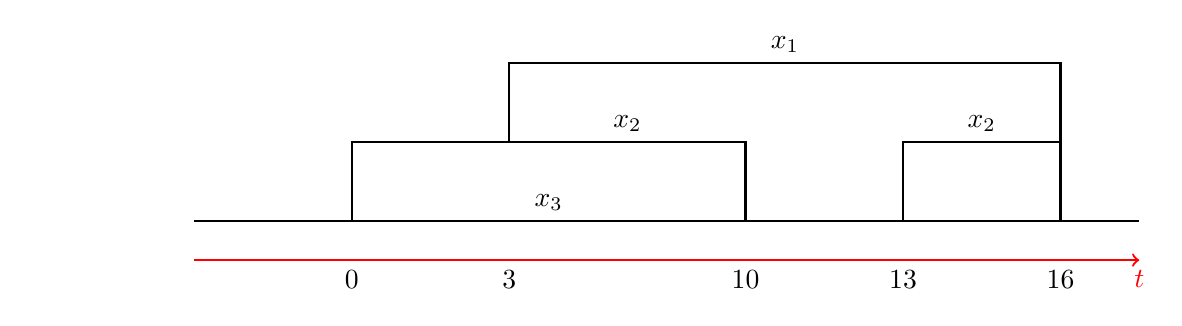
\begin{tikzpicture}[thick]
		\centering
		%%Location
		\draw (-3,0) node {};
		%%axis
		\draw[->][red] (-1,0) -- (11,0) coordinate[label = {below:$t$}] (xmax);
		%%Dendrogram
		\draw plot (1,0.5)--(1,1.5)--(6,1.5)--(6,0.5);
		\draw plot (3,1.5)--(3,2.5)--(10,2.5)--(10,1.5);
		
		\draw plot (8,0.5)--(8,1.5)--(10,1.5)--(10,0.5);
		\draw plot (-1,0.5)--(11,0.5);
		
		
		%%Label
		\draw (1,0) node [anchor=north] {0};
		\draw (3,0) node [anchor=north] {3};
		\draw (6,0) node [anchor=north] {10};
		\draw (8,0) node [anchor=north] {13};
		\draw (10,0) node [anchor=north] {16};
		\draw (6.5,2.5) node [anchor=south] {$x_1$};
		\draw (9,1.5) node [anchor=south] {$x_2$};
		\draw (3.5,0.5) node [anchor=south] {$x_3$};
		\draw (4.5,1.5) node [anchor=south] {$x_2$};
			\end{tikzpicture}
			\caption{Formigram $\theta_X$}
	\end{figure}
	
We obtain a zigzag module $$\mathbb{V}=\mathbb{F}(\theta_X)=\{\mathbb{F}(\theta_X(s))\leftrightarrow \mathbb{F}(\theta_X(t))\}_{s\leq t}$$ by linearizing $\theta_X$.For the sake of simplicity, let $x_i$, $x_{ij}$ and $x_{ijk}$ stand for $\{x_i\}$, $\{x_i,x_j\}$ and $\{x_i,x_j,x_k\}$ respectively. The linear map $f_{9,10}:\mathbb{F}(\theta_X(9))\rightarrow \mathbb{F}(\theta_X(10))$ is defined by 
\begin{align*}
	x_1 &\mapsto x_1\\
	x_2 &\mapsto x_{23}\\
	x_3 &\mapsto x_{23}
\end{align*}
on the canonical basis $\{x_1, x_2, x_3\}$ of $\mathbb{F}(\theta_X(9))$. The linear map $g_{2, 3}:\mathbb{F}(\theta_X(3))\rightarrow \mathbb{F}(\theta_X(2))$ is defined by
\begin{align*}
x_1 &\mapsto x_{12}\\
x_2 &\mapsto x_{12}\\
x_3 &\mapsto x_3
\end{align*}
on the basis $\{x_1, x_2, x_3\}$ of $\mathbb{F}(\theta_X(3))$. But we do not define any map between $\mathbb{F}(\theta_X)(1)$ and $\mathbb{F}(\theta_X)(10)$ because there are two critical values $3, 10$ in $[1,10]$. Now, we choose the basis of $\theta_X(t)$ for each $t\in \mathbb{R}$ as follows:
\begin{itemize}
	\item on $(-\infty,0)\cup[17,\infty)$; $\{x_{123}\}$,
	\item on $[0,3)$; $\{x_{12}-x_3,\ x_3\}$,
	\item on $[3,10)\cup [15,17)$; $\{x_1-x_2,\ x_2-x_3,\ x_3\}$,
	\item on $[10,15)$; $\{x_1-x_{23},\ x_{23}\}$	
\end{itemize}
The following picture illustrates how each basis element flows via linear maps. Especially, the end of a horizontal orbit means the basis element on the orbit is sent to zero by the linear map.

	\begin{figure}[h]
		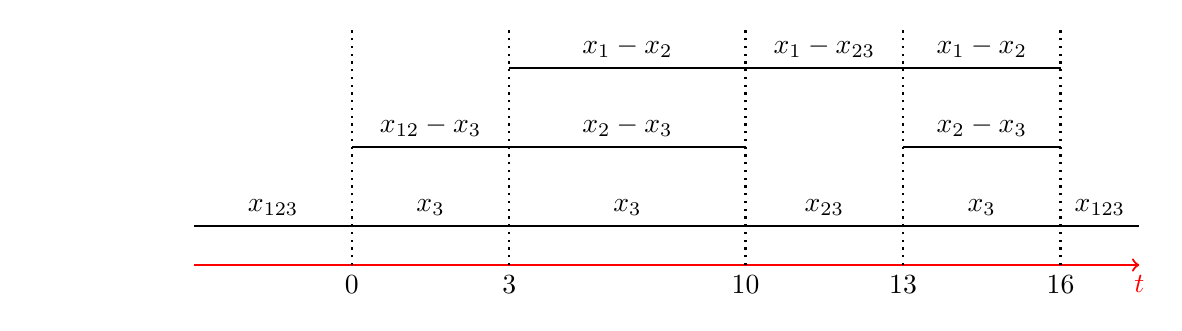
\begin{tikzpicture}[thick]
		\centering
		%%Location
		\draw (-3,0) node {};
		%%axis
		\draw[->][red] (-1,0) -- (11,0) coordinate[label = {below:$t$}] (xmax);
		\draw[dotted] (1,0)--(1,3);
		\draw[dotted] (3,0)--(3,3);
		\draw[dotted] (6,0)--(6,3);
		\draw[dotted] (8,0)--(8,3);
		\draw[dotted] (10,0)--(10,3);
		%%Dendrogram
		\draw plot (1,1.5)--(6,1.5);
		\draw plot (3,2.5)--(10,2.5);
		
		\draw plot (8,1.5)--(10,1.5);
		\draw plot (-1,0.5)--(11,0.5);
		
		
		%%Label
		\draw (1,0) node [anchor=north] {0};
		\draw (3,0) node [anchor=north] {3};
		\draw (6,0) node [anchor=north] {10};
		\draw (8,0) node [anchor=north] {13};
		\draw (10,0) node [anchor=north] {16};
		\draw (7,2.5) node [anchor=south] {$x_1-x_{23}$};
		\draw (4.5,1.5) node [anchor=south] {$x_2-x_3$};
		\draw (4.5,2.5) node [anchor=south] {$x_1-x_2$};
		\draw (4.5,0.5) node [anchor=south] {$x_3$};
		\draw (9,2.5) node [anchor=south] {$x_1-x_2$};
		\draw (9,1.5) node [anchor=south] {$x_2-x_3$};
		\draw (2,1.5) node [anchor=south] {$x_{12}-x_3$};
		\draw (2,0.5) node [anchor=south] {$x_3$};
		\draw (7,0.5) node [anchor=south] {$x_{23}$};
		\draw (0,0.5) node [anchor=south] {$x_{123}$};
		\draw (10.5,0.5) node [anchor=south] {$x_{123}$};
		\draw (9,0.5) node [anchor=south] {$x_3$};
		\end{tikzpicture}
	\end{figure}
	For example, the map $f_{15,17}:\mathbb{F}(\theta_X(15))\rightarrow \mathbb{F}(\theta_X(17))$ can be described by
	\begin{align*}
		x_1-x_2 & \mapsto 0\\
		x_2-x_3 & \mapsto 0\\
		x_3 & \mapsto x_{123}.\\
	\end{align*}
	
	It is clear that the zigzag module $\mathbb{V}$ is isomorphic to $$\mathbb{I}(3,16)\oplus \mathbb{I}(0,10)\oplus \mathbb{I}(13,16)\oplus \mathbb{I}(-\infty,\infty)$$from the picture. 
\end{example}


 
  Given a formigram $\theta_X$, let $C=\{c_1< c_2< \cdots< c_n\}$ be the set of all critical points of $\theta_X$ and take any $c_0\in \mathbb{R}$ which less than $c_1$. Let  $m_k:=\abs{\theta_X(c_k)}$, i.e., the number of blocks in the partition $\theta_X(c_k)$, for $0\leq k \leq n$. Obviously $m_0=1$ by the choice of $c_0$.\\

\no{Step 1.} Draw the graph of $\theta_X$ on the $xy$-plane as follows: Place the block $B_{k,l}\in \theta_X(c_k)$ at $(k,l)$ for all $0\leq k \leq n$ and $1 \leq l \leq m_k$ and all the edges are line segment joining two endpoints such that no edges  cross each other. This requires a proper indexing with respect to $l$ which ranging from 1 to $m_k$ for each $k$ but this must be possible since $\theta_X$ is planar. Observe that for each $1\leq k\leq n-1$ and $1\leq l \leq m_k$, the vertex $B_{k,l}$ must be joined to a vertex $B_{k-1, l_1}$ on the line $x=k-1$ and a vertex $B_{k+1, l_2}$ on the line $x=k+1$.\\

\no{Step 2.} Consider the vector spaces $V_{c_k}=\mathbb{F}(\theta_X(c_k))$ for $0\leq k \leq n$. Choose the basis of $V_{c_k}$ as $\mathcal{B}_{c_k}=\{B_{k,l}-B_{k,l-1}:1\leq l \leq m_k\}$ where $B_{k,0}=0$ as a definition for all $k$.\\ 

\no{Step 3.} For all $t\in (c_k,c_{k+1})$, set up as $\mathcal{B}_{t}=\mathcal{B}_{c_k}$.\\

\begin{example}The following is the graph described in $\mathbf{Step\ 1}$ for the formigram in Example \ref{example}. Also, one can check that this graph matchs Definition \ref{graph}.\footnote{The graph drawing in the described way is not unique depending on the choice of indexing with respect to $l$. But, this choice does not matter.}
	
	\begin{figure}[h]
		\begin{tikzpicture}
			\centering
			%%Location
			\draw (-3,0) node {};
			%%axis
			\draw[->][thick] (-1,0) -- (11,0) coordinate[label = {below:$x$}] (xmax);			
			
			%%Label
			\draw (0,0) node [anchor=north] {0};
		    \draw (2,0) node [anchor=north] {1};
		    \draw (4,0) node [anchor=north] {2};
		    \draw (6,0) node [anchor=north] {3};
		    \draw (8,0) node [anchor=north] {4};
		    \draw (10,0) node [anchor=north] {5};
		    \draw (-0.2,2) node [anchor=south] {$x_{123}$};
		    \draw (1.8,4) node [anchor=south] {$x_{12}$};
		    \draw (2,2) node [anchor=south] {$x_{3}$};
		    \draw (4,2) node [anchor=south] {$x_{3}$};
		    \draw (4,4) node [anchor=south] {$x_{2}$};
		    \draw (4,6) node [anchor=south] {$x_{1}$};
		    \draw (6,2) node [anchor=north] {$x_{23}$};
		    \draw (6,4) node [anchor=north] {$x_{1}$};
		    \draw (8,6) node [anchor=south] {$x_{1}$};
		    \draw (8,4) node [anchor=south] {$x_{2}$};
		    \draw (8,2) node [anchor=south] {$x_{3}$};
		    \draw (10,2) node [anchor=north] {$x_{123}$};
		    \draw (-1.5,2) node {$y=1$};
		    \draw (-1.5,4) node {$y=2$};
		    \draw (-1.5,6) node {$y=3$};
	        \fill (0,2) circle (1.7pt);
		    \fill (2,2) circle (1.7pt);
		    \fill (2,4) circle (1.7pt);
		    \fill (4,2) circle (1.7pt);
		    \fill (4,4) circle (1.7pt);
		    \fill (4,6) circle (1.7pt);
		    \fill (6,2) circle (1.7pt);
		    \fill (6,4) circle (1.7pt);
		    \fill (8,2) circle (1.7pt);
		    \fill (8,4) circle (1.7pt);
		    \fill (8,6) circle (1.7pt);
		    \fill (10,2) circle (1.7pt);
		    \draw (0,2)--(10,2);
		    \draw (0,2)--(4,6);
		    \draw (2,4)--(4,4)--(6,2)--(8,4)--(10,2);
		    \draw (4,6)--(6,4)--(8,6)--(10,2);
		    \draw[dotted] (-1,2)--(0,2);
		    \draw[dotted] (-1,4)--(10,4); 
		    \draw[dotted] (-1,6)--(10,6);
		    
		\end{tikzpicture}
	\end{figure} 
	
\end{example}

\begin{proposition} The collection $\mathcal{B}=\{\mathcal{B}_t\}_{t\in\mathbb{R}}$ is the basis of the zigzag module $\mathbb{V}=\mathbb{F}(\theta_X)$
\begin{proof}
	Take any  $\eps\in (0,\delta)$ where $\displaystyle \delta= \min_{1\leq k \leq n}\abs{c_k-c_{k-1}}. $
	It suffices to prove that each matrix of linear maps, either $$g_{c_k-\eps}:V_{c_k}\rightarrow V_{c_k-\eps}\ \mbox{when $\theta_X(c_k)$ is finer than $\theta_X(c_k-\eps)$}$$ or $$f_{c_k-\eps}:V_{c_k-\eps}\rightarrow V_{c_k} \ \mbox{when $\theta_X(c_k)$ is coarser than $\theta_X(c_k-\eps)$}$$ with respect to the bases $\mathcal{B}_{c_k-\eps}$ and $\mathcal{B}_{c_k}$ is a matrix of matching for each $k$, i.e, every component is either 0 or 1 and there could be at most one 1 in each row and column. \footnote{For any $c_k\leq s< t <c_{k+1}$, the matrix of $f_{s}:V_s\rightarrow V_t$ is the identity matix and hence it is a matrix of matching.}\\
	
	
	In either cases of these the proof are identical so fix $1\leq k\leq n$ and assume that $\theta_X(c_k)$ is coarser than $\theta_X(c_k-\eps)$. By \textbf{Step 3}, $\mathcal{B}_{c_k-\eps}=\mathcal{B}_{c_{k-1}}$. Pick any $1\leq l \leq m_{k-1}$. If $B_{k-1,l}, B_{k-1,l-1}\in \theta_X(c_k-\eps)$ come together at time $c_k$, then $$f_{c_k-\eps}(B_{k-1,l}-B_{k-1,l-1})=0$$ which implies that the $l$-th column of the matrix of $f_{c_k-\eps}$ is zero. Suppose that $B_{k-1,l}$ and  $B_{k-1,l-1}$ do not merge at time $c_k$. Then $$f_{c_k-\eps}(B_{k-1,l})=B_{k,\alpha}\ \ \mbox{and}\ \ f_{c_k-\eps}(B_{k-1,l-1})=B_{k,\beta}$$ where $\alpha\neq \beta$. We claim that $\alpha-\beta=1$, meaning that the $l$-th column contains exactly one $1$. First, $\alpha-\beta$ cannot be negative since no edges in the graph of $\theta_X$ drawn in \textbf{Step 1} cross. Now assume that $\alpha-\beta\geq 2.$ Then the vertex $B_{k,\alpha-1}$, which is located lower than $B_{k,\alpha}$ and higher than $B_{k,\beta}$ on the line $x=k$, cannot be joined by any vertex on the line $x=k-1$ by noncrossing property of the graph drawn in \textbf{Step 1}, which contradicts the observation described in \textbf{Step 1}. (See the Figure 12.)
	
	\begin{center}
		\begin{figure}[h]
			\begin{tikzpicture}
			\draw (-6.5,0) node {};
			\fill (0,2) circle (1.7pt);
			\fill (0,3) circle (1.7pt);
			\fill (2,2) circle (1.7pt);
			\fill (2,1) circle (1.7pt);
			\fill (2,0) circle (1.7pt);
			\fill (0,4) circle (1.7pt);
			\fill (0,-1) circle (1.7pt);
			\fill (0,1) circle (1.7pt);
			\draw[dotted] (0,-2)--(0,4); 
			\draw[dotted] (2,-2)--(2,4); 
			\draw (0.8,2) node {$B_{k-1,l-1}$};
			\draw (0.5,3.2) node {$B_{k-1,l}$};
			\draw (0,-2) node [anchor=north] {$k-1$};
			\draw (2,-2) node [anchor=north] {$k$};
			\draw (5.5,-2) node [anchor=north] {$x$};
			\draw (2.5,2) node {$B_{k,\alpha}$};
			\draw (2.65,1) node {$B_{k,\alpha-1}$};
			\draw (2.5,0) node {$B_{k,\beta}$};
			\draw[red] (-1,1)--(0,2)--(2,0)--(3,-1);
			\draw[red] (-1,2)--(0,3)--(2,2)--(3,1);
			\draw[red] (-1,0)--(0,1)--(1,0);
			\draw[red] (-1,-1)--(0,-1)--(1,-1);
			\draw[red] (-1,3)--(0,4)--(1,3.5);
			\draw[->] (-2.5,-2) -- (5,-2);
			\draw (0,0) node {$\approx$};
			\end{tikzpicture} 
			\caption{If $B_{k-1,l}$ and $B_{k-1,l-1}$ are joined by ${B_{k,\alpha}}$ and $B_{k,\beta}$ respectively where $\alpha-\beta\geq 2$, then $B_{k,\alpha-1}$ cannot be connected to a vertex on the line $x=k-1$ without enforcing the edge shooting from $B_{k,\alpha-1}$ to intersect an edge.}
		\end{figure}
	\end{center}
	
	It remains to prove that each row of the matrix contains at most one $1$. To this end, assume that there are $1\leq l_1\leq l_2 \leq m_{k-1}$ such that 
	$$f_{c_k-\eps}(B_{k-1,l_1}-B_{k-1,l_1-1})=f_{c_k-\eps}(B_{k-1,l_2}-B_{k-1,l_2-1})=B_{k,\alpha}-B_{k,\alpha-1}.$$
	Then only possible action of $f_{c_k-\eps}$ on $\{B_{k-1,l_1},\ B_{k-1,l_1-1},\ B_{k-1,l_2},\ B_{k-1,l_2-1}\}$ is
	\begin{center}
		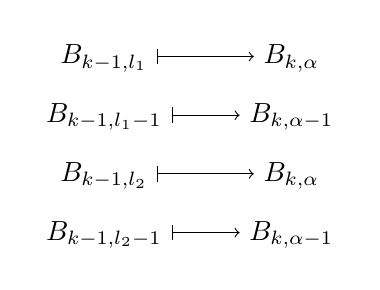
\begin{tikzpicture}
		\matrix(a)[matrix of math nodes,
		row sep=0.7em, column sep=2.5em,
		text height=1.5ex, text depth=0.25ex]
		{B_{k-1,l_1}&B_{k,\alpha}\\B_{k-1,l_1-1}&B_{k,\alpha-1}\\B_{k-1,l_2}&B_{k,\alpha}\\B_{k-1,l_2-1}&B_{k,\alpha-1}\\};
		\path[|->,font=\scriptsize]
		(a-1-1) edge (a-1-2);
		\path[|->,font=\scriptsize]
		(a-2-1) edge (a-2-2);
		\path[|->,font=\scriptsize]
		(a-3-1) edge (a-3-2);
		\path[|->,font=\scriptsize]
		(a-4-1) edge (a-4-2);	
		\end{tikzpicture}
	\end{center}
	with it in mind that the graph drawn in \textbf{Step 1} does not have any crossing edges. Notice that $B_{k-1,l_1}$ and $B_{k-1,l_2}$ merge to form $B_{k,\alpha}$ whereas $B_{k-1,l_2-1}$ become a part of $B_{k,\alpha-1}$ at time $c_k$. (See Figure 13). 
	
	\begin{center}
		\begin{figure}[h]
			\begin{tikzpicture}
			\draw (-6.5,0) node {};
			\fill (0,1.7) circle (1.7pt);
			\fill (0,2.7) circle (1.7pt);
			\fill (2,-0.2) circle (1.7pt);
			\fill (2,-1.2) circle (1.7pt);
			\fill (0,-1) circle (1.7pt);
			\fill (0,0) circle (1.7pt);
			\draw[dotted] (0,-2)--(0,3); 
			\draw[dotted] (2,-2)--(2,3); 
			\draw (-1,1.7) node {$B_{k-1,l_2-1}$};
			\draw (-0.7,2.7) node {$B_{k-1,l_2}$};
			\draw (-0.7,0) node {$B_{k-1,l_1}$};
			\draw (-1,-1) node {$B_{k-1,l_1-1}$};
			\draw (0,-2) node [anchor=north] {$k-1$};
			\draw (2,-2) node [anchor=north] {$k$};
			\draw (5.5,-2) node [anchor=north] {$x$};
			\draw (2.5,-0.2) node {$B_{k,\alpha}$};
			\draw (2.65,-1.2) node {$B_{k,\alpha-1}$};
			\draw[red] (0,1.7)--(2,-1.2);
			\draw[red] (0,2.7)--(2,-0.2);
			\draw[red] (0,0)--(2,-0.2);
			\draw[red] (0,-1)--(2,-1.2);
			\draw[->] (-2.5,-2) -- (5,-2);
			\draw (0,0.7) node {$\approx$};
			\end{tikzpicture} 
			\caption{}
		\end{figure}
	\end{center}
	If $l_2-1>l_1$, the above Figure certainly contains crossing edges. Further, $l_2-1$ cannot be equal to  $l_1$ since $B_{k-1,l_2-1}$ and $B_{k-1,l_1}$ do not merge at time $c_k$. Eventually, we conclude that $l_2=l_1$ and this implies that the matrix of $f_{{c_k}-\eps}$ cannot have more than two 1s in a row as desired.
\end{proof}
\end{proposition} 	

\subsubsection{Relationship between the set-theoretic diagrams and the algebraic diagrams}
It turns out that there are many cases where the algebraic diagram coincides with a set-theoretic diagram by assigning a proper order on the underlying set. Nevertheless, some formigrams $\theta_X$ cannot attain any order $\mathfrak{o}_X$ on $X$ whose the set-theoretic diagram of $\mathcal{X}=(X,\theta_X,\mathfrak{o}_X)$ is identical to $\dgm(\mathbb{F}(\theta_X))$. Here is a simple example of this case.

\begin{example} \label{example5.3}Consider the formigram as Figure 14 with twelve critical values $$c_1=10<11< \cdots< 23=c_{12}.$$	
	\begin{center}
		\begin{figure}[h]
			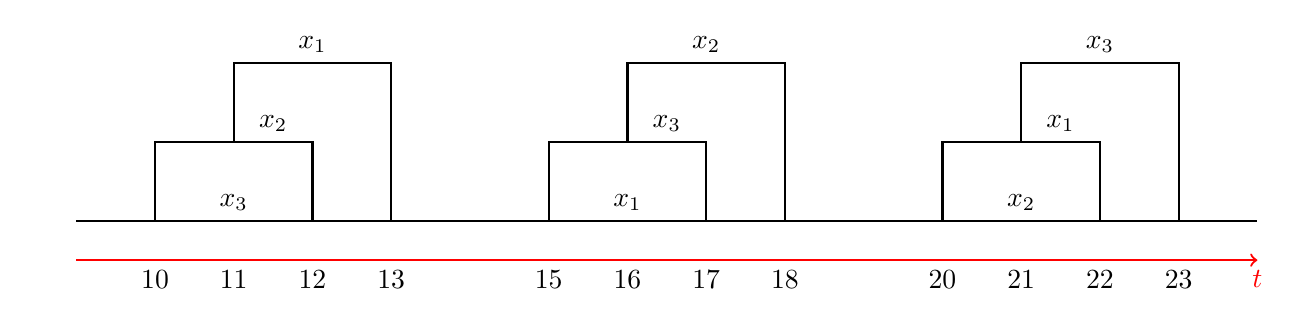
\begin{tikzpicture}[thick]
			\centering
			%%Location
			\draw (-2.5,0) node {};
			%%axis
			\draw[->][red] (-2,0) -- (13,0) coordinate[label = {below:$t$}] (xmax);
			%%Dendrogram
			\draw plot (-1,0.5)--(-1,1.5)--(1,1.5)--(1,0.5);
			\draw plot (0,1.5)--(0,2.5)--(2,2.5)--(2,0.5);
			\draw plot (4,0.5)--(4,1.5)--(6,1.5)--(6,0.5);
			\draw plot (5,1.5)--(5,2.5)--(7,2.5)--(7,0.5);
			
			\draw plot (9,0.5)--(9,1.5)--(11,1.5)--(11,0.5);
			\draw plot (10,1.5)--(10,2.5)--(12,2.5)--(12,0.5);
			\draw plot (-2,0.5)--(13,0.5);
			
			
			%%Label
			\draw (-1,0) node [anchor=north] {10};
			\draw (0,0) node [anchor=north] {11};
			\draw (1,0) node [anchor=north] {12};
			\draw (2,0) node [anchor=north] {13};
			\draw (4,0) node [anchor=north] {15};
			\draw (5,0) node [anchor=north] {16};
			\draw (6,0) node [anchor=north] {17};
			\draw (7,0) node [anchor=north] {18};
			\draw (9,0) node [anchor=north] {20};
			\draw (11,0) node [anchor=north] {22};
			\draw (10,0) node [anchor=north] {21};
			\draw (12,0) node [anchor=north] {23};
			\draw (1,2.5) node [anchor=south] {$x_1$};
			\draw (6,2.5) node [anchor=south] {$x_2$};
			\draw (5,0.5) node [anchor=south] {$x_1$};
			\draw (0.5,1.5) node [anchor=south] {$x_2$};
			\draw (0,0.5) node [anchor=south] {$x_3$};
			\draw (5.5,1.5) node [anchor=south] {$x_3$};
			\draw (10.5,1.5) node [anchor=south] {$x_1$};
			\draw (11,2.5) node [anchor=south] {$x_3$};
			\draw (10,0.5) node [anchor=south] {$x_2$};
			\end{tikzpicture}\caption{Formigram $\theta_X$}
			\end{figure}
			
	\end{center}
	
	It is not difficult to check that Figure 15 is the graph on $xy$-plane of this formigram with natural ordering on each partition as Figure 13 indicates. 


\begin{figure}
	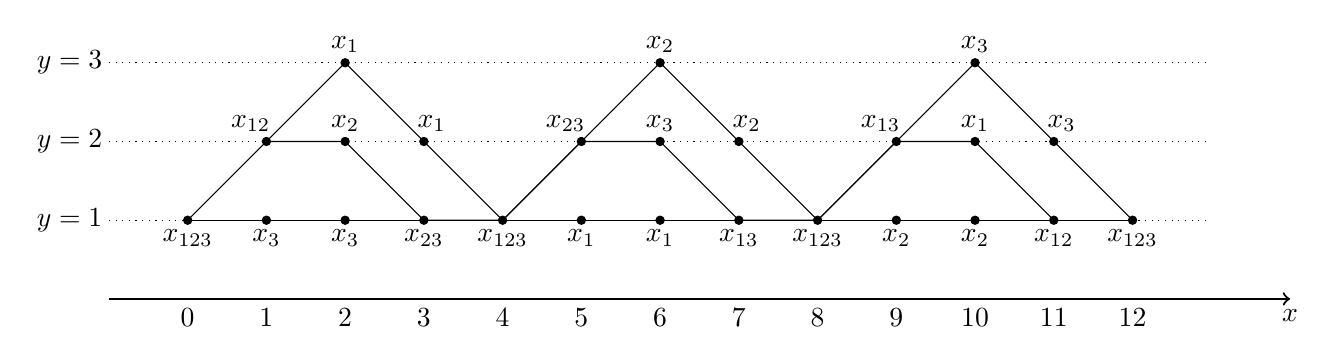
\begin{tikzpicture}
	
		\centering
		%%Location
		\draw (-1.5,0) node {};
		%%axis
		\draw[->][thick] (-2,0) -- (13,0) coordinate[label = {below:$x$}] (xmax);			
		
		%%Label
		\draw (-1,0) node [anchor=north] {0};
		\draw (0,0) node [anchor=north] {1};
		\draw (1,0) node [anchor=north] {2};
		\draw (2,0) node [anchor=north] {3};
		\draw (3,0) node [anchor=north] {4};
		\draw (4,0) node [anchor=north] {5};
		\draw (5,0) node [anchor=north] {6};
		\draw (6,0) node [anchor=north] {7};
		\draw (7,0) node [anchor=north] {8};
		\draw (8,0) node [anchor=north] {9};
		\draw (9,0) node [anchor=north] {10};
		\draw (10,0) node [anchor=north] {11};
		\draw (11,0) node [anchor=north] {12};
		\draw (-1,1) node [anchor=north] {$x_{123}$};
		\draw (0,1) node [anchor=north] {$x_{3}$};
		\draw (-0.2,2) node [anchor=south] {$x_{12}$};
		\draw (1,2) node [anchor=south] {$x_{2}$};
		\draw (1,3) node [anchor=south] {$x_{1}$};
		\draw (1,1) node [anchor=north] {$x_{3}$};
		\draw (2,1) node [anchor=north] {$x_{23}$};
		\draw (2.1,2) node [anchor=south] {$x_{1}$};
		\draw (3,1) node [anchor=north] {$x_{123}$};
		\draw (4,1) node [anchor=north] {$x_{1}$};
		\draw (3.8,2) node [anchor=south] {$x_{23}$};
		\draw (5,1) node [anchor=north] {$x_{1}$};
		\draw (5,2) node [anchor=south] {$x_{3}$};
		\draw (5,3) node [anchor=south] {$x_{2}$};
		\draw (6,1) node [anchor=north] {$x_{13}$};
		\draw (6.1,2) node [anchor=south] {$x_{2}$};
		\draw (7,1) node [anchor=north] {$x_{123}$};
		\draw (8,1) node [anchor=north] {$x_{2}$};
		\draw (7.8,2) node [anchor=south] {$x_{13}$};
	    \draw (9,1) node [anchor=north] {$x_{2}$};
	    \draw (9,2) node [anchor=south] {$x_{1}$};
	    \draw (9,3) node [anchor=south] {$x_{3}$};
	    \draw (10.1,2) node [anchor=south] {$x_{3}$};
	    \draw (10,1) node [anchor=north] {$x_{12}$};
	    \draw (11,1) node [anchor=north] {$x_{123}$};
				
		
	
		\fill (-1,1) circle (1.7pt);
		\fill (0,1) circle (1.7pt);
		\fill (0,2) circle (1.7pt);
		\fill (1,1) circle (1.7pt);
		\fill (1,2) circle (1.7pt);
		\fill (1,3) circle (1.7pt);
		\fill (2,1) circle (1.7pt);
		\fill (3,1) circle (1.7pt);
		\fill (4,1) circle (1.7pt);
		\fill (4,2) circle (1.7pt);
		\fill (5,3) circle (1.7pt);
		\fill (5,1) circle (1.7pt);
		\fill (6,1) circle (1.7pt);
		\fill (6,2) circle (1.7pt);
		\fill (7,1) circle (1.7pt);
		\fill (9,3) circle (1.7pt);
		\fill (8,1) circle (1.7pt);
		\fill (9,1) circle (1.7pt);
		\fill (9,2) circle (1.7pt);
		\fill (10,1) circle (1.7pt);
		\fill (10,2) circle (1.7pt);
		\fill (11,1) circle (1.7pt);
		\fill (2,2) circle (1.7pt);
		\fill (5,2) circle (1.7pt);
		\fill (8,2) circle (1.7pt);
		
		
		\draw (-1,1)--(1,3)--(2,2)--(3,1)--(5,3)--(7,1)--(9,3)--(11,1);
		\draw (0,2)--(1,2)--(2,1)--(3,1)--(4,2)--(5,2)--(6,1)--(7,1)--(8,2)--(9,2)--(10,1);
		\draw (-1,1)--(11,1);		
		\draw[dotted] (-2,1)--(12,1);
		\draw[dotted] (-2,2)--(12,2); 
		\draw[dotted] (-2,3)--(12,3);
		
		\draw (-2.5,1) node {$y=1$};
		\draw (-2.5,2) node {$y=2$};
		\draw (-2.5,3) node {$y=3$};		
	\end{tikzpicture}	
	\caption{The graph of $\theta_X$ on the $xy$-plane. }
\end{figure}

When once the pictorial graph illustrating the stratified structure of formigram like Figure 14 is drawn, the choice of basis for $\mathbb{F}(\theta_X(t))$ automatically follows as described in \textbf{Step 2}, and \textbf{Step 3} which yields the the basis of the entire zigzag module $\mathbb{F}(\theta_X)$.\footnote{If a formigram is given by a picture like Figure 13, i.e., a planary picture with stratified structure, it is not necessary in fact to draw the graph of it to obtain a basis for $\mathbb{F}(\theta_X)$. %Regarding each row as a floor, (the element on $i$-th floor)$-$(the element on $i-1$-th floor) yields a proper basis for all $i$ across all the time $t$.  
However, we would not get the formigram as a picture from the real world in general and we have to stratify the structure by drawing the graph in a standard way as suggested before in that case.} For instance, the basis for $\mathbb{F}(\theta_X(c_6))=\mathbb{F}(\theta_X(16))$ would be chosen as an ordered basis $\{x_2-x_3, x_3-x_1, x_1\}$. The following picture illustrates not only how each orbit looks like but also the choice of basis across all the time.
	\begin{center}
		\begin{figure}[h]
			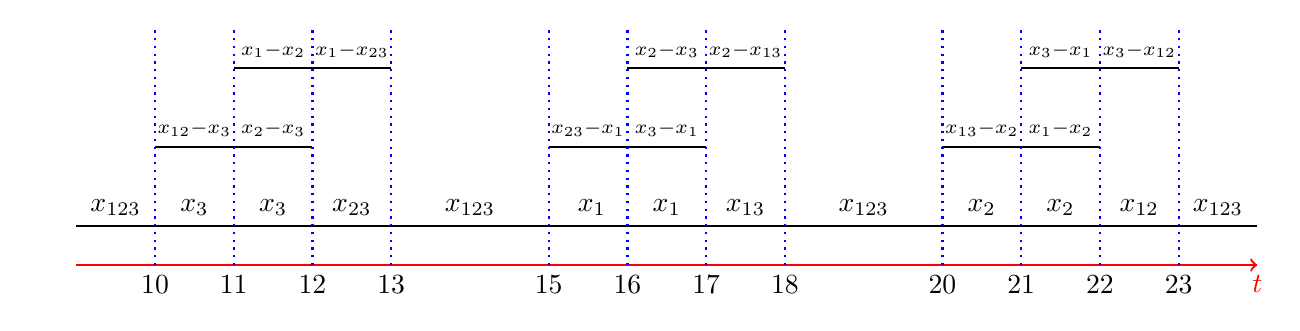
\begin{tikzpicture}[thick]
			\centering
			%%Location
			\draw (-2.5,0) node {};
			%%axis
			\draw[->][red] (-2,0) -- (13,0) coordinate[label = {below:$t$}] (xmax);
			%%Dendrogram
			\draw plot (-1,1.5)--(1,1.5);
			\draw plot (0,2.5)--(2,2.5);
			\draw plot (4,1.5)--(6,1.5);
			\draw plot (5,2.5)--(7,2.5);			
			\draw plot (9,1.5)--(11,1.5);
			\draw plot (10,2.5)--(12,2.5);
			\draw plot (-2,0.5)--(13,0.5);
			\draw[dotted, blue] (-1,0)--(-1,3);
			\draw[dotted, blue] (0,0)--(0,3); 
			\draw[dotted, blue] (1,0)--(1,3); 
			\draw[dotted, blue] (2,0)--(2,3); 
			\draw[dotted, blue] (4,0)--(4,3); 
			\draw[dotted, blue] (5,0)--(5,3); 
			\draw[dotted, blue] (6,0)--(6,3);
			\draw[dotted, blue] (7,0)--(7,3); 
			\draw[dotted, blue] (9,0)--(9,3); 
			\draw[dotted, blue] (10,0)--(10,3); 
			\draw[dotted, blue] (11,0)--(11,3); 			
			\draw[dotted, blue] (12,0)--(12,3); 
			 
			
			%%Label
			\draw (-1,0) node [anchor=north] {10};
			\draw (0,0) node [anchor=north] {11};
			\draw (1,0) node [anchor=north] {12};
			\draw (2,0) node [anchor=north] {13};
			\draw (4,0) node [anchor=north] {15};
			\draw (5,0) node [anchor=north] {16};
			\draw (6,0) node [anchor=north] {17};
			\draw (7,0) node [anchor=north] {18};
			\draw (9,0) node [anchor=north] {20};
			\draw (11,0) node [anchor=north] {22};
			\draw (10,0) node [anchor=north] {21};
			\draw (12,0) node [anchor=north] {23};
			\draw (0.5,2.5) node [anchor=south] {$\scriptstyle{x_1-x_2}$};
			\draw (5.5,2.5) node [anchor=south] {$\scriptstyle{x_2-x_3}$};
			\draw (1.5,2.5) node [anchor=south] {$\scriptstyle{x_1-x_{23}}$};
			\draw (6.5,2.5) node [anchor=south] {$\scriptstyle{x_2-x_{13}}$};
			\draw (1.5,0.5) node [anchor=south] {$x_{23}$};
			\draw (6.5,0.5) node [anchor=south] {$x_{13}$};
			\draw (-0.5,1.5) node [anchor=south] {$\scriptstyle{x_{12}-x_3}$};
			\draw (4.5,1.5) node [anchor=south] {$\scriptstyle{x_{23}-x_1}$};
			\draw (9.5,1.5) node [anchor=south] {$\scriptstyle{x_{13}-x_2}$};
			\draw (9.5,0.5) node [anchor=south] {${x_{2}}$};
			\draw (10.5,0.5) node [anchor=south] {${x_{2}}$};
			\draw (-1.5,0.5) node [anchor=south] {$x_{123}$};
			\draw (3,0.5) node [anchor=south] {$x_{123}$};
			\draw (8,0.5) node [anchor=south] {$x_{123}$};
			\draw (4.55,0.5) node [anchor=south] {$x_1$};
			\draw (5.5,0.5) node [anchor=south] {$x_1$};
			\draw (0.5,1.5) node [anchor=south] {$\scriptstyle{x_2-x_3}$};
			\draw (-0.5,0.5) node [anchor=south] {$x_3$};
			\draw (0.5,0.5) node [anchor=south] {$x_3$};
			\draw (5.5,1.5) node [anchor=south] {$\scriptstyle{x_3-x_1}$};
			\draw (10.5,1.5) node [anchor=south] {$\scriptstyle{x_1-x_2}$};
			\draw (11.5,0.5) node [anchor=south] {$x_{12}$};
			\draw (10.5,2.5) node [anchor=south] {$\scriptstyle{x_3-x_1}$};
			\draw (11.5,2.5) node [anchor=south] {$\scriptstyle{x_3-x_{12}}$};
			\draw (12.5,0.5) node [anchor=south] {$x_{123}$};
			\end{tikzpicture}\caption{Formigram $\theta_X$}
		\end{figure}		
	\end{center}Finally, we get $$\mathbb{F}(\theta_X)\simeq \mathbb{I}(10,12)\oplus\mathbb{I}(11,13)\oplus\mathbb{I}(15,17)\oplus\mathbb{I}(16,18)\oplus\mathbb{I}(20,22)\oplus\mathbb{I}(21,23)\oplus\mathbb{I}(-\infty,\infty).$$ However, regardless of the choice of order on $X$, one can check that the set-theoretic diagram contains one of $[11,12), [16,17)$ or $[21,22)$, which do not belong to the algebraic diagram.
		\end{example}

We introduce hierarchical structure of the class of formigrams.

\begin{definition} To say that a formigram $\theta_X$ is algebraic means that there exists an order $\mathfrak{o}_X$ on $X$ such that $$\dgm(\mathcal{X})=\dgm(\mathbb{F}(\theta_X))$$ for $\mathcal{X}=(X,\theta_X, \mathfrak{o}_X)$.
\end{definition}

\begin{definition} \label{stratifiable}To say that a formigram $\theta_X$ is stratifiable (by an order) means that there exists an order $\mathfrak{o}_X$ on $X$ such that the graph of $\theta_X$ drawn in the following manner on $xy$-plane is planar: Let $c_1<\cdots<c_n$ be critical values of $\theta_X$ and take any $c_0<c_1$. Let $m_k=\abs{\theta_X(c_k)}$ for $0\leq k\leq n$. Place the block $B_{k,l}\in \theta_X(c_k)$ at $(k,l)$  so that $$\max B_{k,l_1}< \max B_{k,l_2} \Rightarrow l_1< l_2.$$ for all $0\leq k \leq n$ and $1 \leq l \leq m_k$
\end{definition}		
	
\begin{example} The formigram in Example \ref{example5.3} is not stratifiable by an order. Indeed, it is easy to check that the graph cannot be drawn meeting the condition in Definition \ref{stratifiable} whatever an order is assigned on the underlying set: For example, if we have $(X,\mathfrak{o}_X)=\{x_3<x_1< x_2\}$, then the left beginning part of the graph,  from $x=0$ to $x=4$, should look as Figure 16, which contains crossing edges. Similarly, even if $X$ attains any different order, there are two edges crossing each other between [$x=2$ and $x=3$], [$x=6$ and $x=7$] or [$x=10$ and $x=11$] when the graph is drawn according to the rule in Definition \ref{stratifiable}. 
	\begin{figure}[h]
		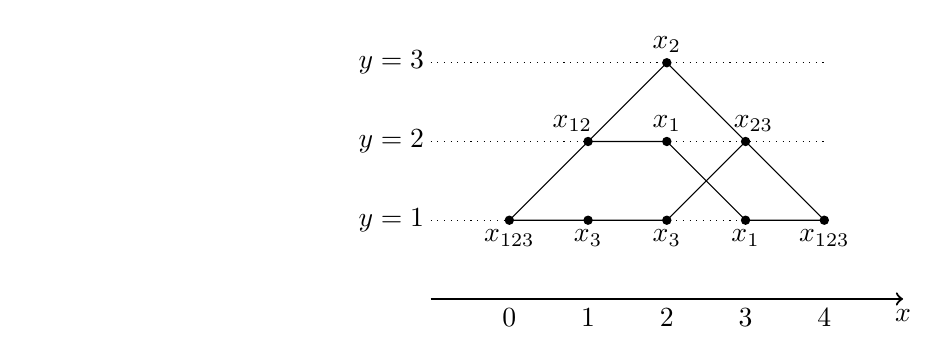
\begin{tikzpicture}
		
		\centering
		%%Location
		\draw (-7,0) node {};
		%%axis
		\draw[->][thick] (-2,0) -- (4,0) coordinate[label = {below:$x$}] (xmax);			
		
		%%Label
		\draw (-1,0) node [anchor=north] {0};
		\draw (0,0) node [anchor=north] {1};
		\draw (1,0) node [anchor=north] {2};
		\draw (2,0) node [anchor=north] {3};
		\draw (3,0) node [anchor=north] {4};

		
		\draw (-1,1) node [anchor=north] {$x_{123}$};
		\draw (0,1) node [anchor=north] {$x_{3}$};
		\draw (-0.2,2) node [anchor=south] {$x_{12}$};
		\draw (1,2) node [anchor=south] {$x_{1}$};
		\draw (1,3) node [anchor=south] {$x_{2}$};
		\draw (1,1) node [anchor=north] {$x_{3}$};
		\draw (2,1) node [anchor=north] {$x_{1}$};
		\draw (2.1,2) node [anchor=south] {$x_{23}$};
		\draw (3,1) node [anchor=north] {$x_{123}$};	
		
		\fill (-1,1) circle (1.7pt);
		\fill (0,1) circle (1.7pt);
		\fill (0,2) circle (1.7pt);
		\fill (1,1) circle (1.7pt);
		\fill (1,2) circle (1.7pt);
		\fill (1,3) circle (1.7pt);
		\fill (2,1) circle (1.7pt);
		\fill (2,2) circle (1.7pt);
		\fill (3,1) circle (1.7pt);
	
		\draw (-1,1)--(1,3)--(2,2)--(3,1);
		\draw (0,2)--(1,2)--(2,1)--(3,1);
		\draw (-1,1)--(1,1)--(2,2);		
		\draw[dotted] (-2,1)--(3,1);
		\draw[dotted] (-2,2)--(3,2); 
		\draw[dotted] (-2,3)--(3,3);
		
		\draw (-2.5,1) node {$y=1$};
		\draw (-2.5,2) node {$y=2$};
		\draw (-2.5,3) node {$y=3$};		
		\end{tikzpicture}	
		\caption{The graph of $\theta_X$ on the $xy$-plane. }
	\end{figure}
	
	
	
\end{example}


\begin{definition} To say that a formigram $\theta_X$ is interval means that there exists an order $\mathfrak{o}_X$ on $X$ such that $\theta_X(t)$ only consists of blocks of consecutive elements by the order $\mathfrak{o}_X$.
\end{definition}	
	
we denote the class of planary formigrams, the class of algebraic, stratifiable and interval formigrams by $\mathcal{F}_{\mathrm{planar}}$, $\mathcal{F}_{\mathrm{algebraic}}$, $\mathcal{F}_{\mathrm{stratifiable}}$ and $\mathcal{F}_{\mathrm{interval}}$ respectively.


\begin{proposition} (tentative) $\mathcal{F}_{\mathrm{planar}}\supset \mathcal{F}_{\mathrm{algebraic}}\supset \mathcal{F}_{\mathrm{stratifiable}}\supset \mathcal{F}_{\mathrm{interval}}$.\\
\begin{proof}\no{Proof for $\mathcal{F}_{\mathrm{planar}}\supset \mathcal{F}_{\mathrm{algebraic}}$}: A formigram given in Example 5.3 is an example which belongs to $\mathcal{F}_{\mathrm{planar}}$ but $ \mathcal{F}_{\mathrm{algebraic}}$ \woojin{However, still not sure whether every algebraic formigram is planar. It suffices to show that every non-planar is not algebraic. I have worked on Zane's non-planary example and it turns out that it is not algebraic, which is nice signal for my conjecture. $K_5$ cannot be contained in the graph of formigram since the graph of formigram does not contain a triangle. So, we only need to ponder on how $K_{3,3}$ in the graph of formigram affects the algebraic diagram.}\\
	
\no{Proof for $\mathcal{F}_{\mathrm{algebraic}}\supset \mathcal{F}_{\mathrm{stratifiable}}$} : Let $\theta_X$ be a stratifiable forgmigram and pick a proper order $\mathfrak{o}_X$ as in Definition \ref{stratifiable}. Now, we claim that $\dgm(\mathcal{X})\subseteq\dgm(\mathbb{F}(\theta_X))$. Let $I\in \dgm(\mathcal{X})=\bigcupdot_{x\in X} \dgm(\mathcal{X},x)$. Then there exists $x\in X$ such that $I\in \dgm(\mathcal{X},x)$, which means that $x$ is the dominating element in the block containing it on the time interval $I=[a,b)$. Especially, since $x$ was not the dominating element right before the time $a$, the branching process occurs at the time $a$. The terminal of dominance of $x$ at time $b$ also implies that the merging must occur at time $b$. Now, look at the graph of $\theta_X$ with respect to the order $\mathfrak{o}_X$ as in Definition $\ref{stratifiable}$. Letting $a=c_k$ and $[x]_{c_k}=B_{k,l}$, we would have $B_{k,l}-B_{k,l-1}$ as a basis element of $\mathcal{B}_{c_k}$. It is easy to check that the orbit of $B_{k,l}-B_{k,l-1}$ in the zigzag module $\mathbb{F}(\theta_X)$ is isomorphic to $\mathbb{I}(a,b)$ and hence $I=[a,b)\in \dgm(\mathbb{F}(\theta_X))$.\\

Conversely, assume that $I=[a,b)=[c_k,c_l)\in \dgm(\mathbb{F}(\theta_X))$ where $k<l$ which is an interval for the orbit of $B_{k,l}-B_{k,l-1}$ for some $1\leq l\leq m_k$. This implies that the maxima of $B_{k,l}$ and $B_{k,l-1}$ are separate on the time interval $[a,b)$ and belong to the same block at $t=a-\eps$ and $t=b+\eps$ for small enough $\eps>0$. This exactly tells us that $$I\in \dgm(\mathcal{X}, x) \subset \dgm(\mathcal{X})$$ for which $x=\max B_{k,l-1}$.\\


\no{Proof for $\mathcal{F}_{\mathrm{stratifiable}}\supset \mathcal{F}_{\mathrm{interval}}$} : Let $\theta_X$ be an interval formigram with a proper order on $X$, say $\{x_1< x_2< \cdots, x_n\}$, so that each blocks are intervals with respect to this order. Draw the graph of $\theta_X$ in the way described in Definition \ref{stratifiable}. Then it is easy to see that the graph does not have any crossing edges.

\woojin{By the second and the third claims, every interval formigram is algebraic.}


\end{proof}
		


\end{proposition}	
	
\newpage 
\section{Computational details and experiments}

\subsection{Curves on the space of metric spaces}

We are going to define a metric $D$ between curves $\gamma, \gamma':[0,1]\rightarrow \mathcal{M}$ on the space of metric spaces. Let $C_{\delta}$ be a Single Linkage Clustering with parameter $\delta>0$. $C_{\delta}\circ \gamma$ and $C_{\delta}\circ \gamma'$ are formigrams and we had defined a distance 'dist' between two formigrams. The goal of this paper is to show the stability result: $$D(\gamma, \gamma')\geq \mathrm{dist}(C_{\delta}\circ \gamma, C_{\delta'}\circ \gamma')$$


\begin{definition} Let $\gamma, \gamma':[0,1]\rightarrow \mathcal{M}$ be two curves on the space $\mathcal{M}$ of metric spaces such that $\gamma(1)=\gamma'(1)=\{*\}$ where $\{*\}$ stands for one-point metric space.
We define 

$$D(\gamma, \gamma'):=\inf_{\alpha,\beta}\max_{0\leq t\leq 1}\{\abs{t-\alpha(t)}, \abs{t-\beta(t)}\}$$
where the infimum is taken over all $\alpha:[0,1]\rightarrow [0,1]$, $\beta:[0,1]\rightarrow [0,1]$ suth that 

\begin{itemize}
	\item $\alpha(t)\geq t$ and $\beta(t)\geq t$ for all $t\in[0,1]$
	\item $d_X(t)(x,x')\geq d_Y(\alpha(t))(x,x')$
	\item $d_Y(t)(y,y')\geq d_X(\beta(t))(x,x')$
\end{itemize}
	\bibliographystyle{plain}
	\nocite{*}
	\bibliography{Formigram_bib}

\end{definition}

\subsection{Reeb graph like constructions}
\facundo{please fill in}

\subsection{Dynamical clustering}
Just assume you have a finite metric space $(X,d_X)$ and a (continuous) function $\delta:[0,\infty) \rightarrow [0,\infty)$. Then define the formigram $\theta_X(t):= C_{\delta(t)}(X,d_X)$. This case may arise when a given fixed configuration of points (say cities) undergoes different connectivity situations: the cities are linked by radio channels whose capacity fluctuates with time. Then, depending on say weather conditions, certain subgroups of cities may become isolated from other subgroups etc, and then these may be linked a a later time. I imagine that this scenario somehow arises in biology when one studies the interaction between organisms which are somehow bound to live in certain fixed areas.

At any rate, the question is whether these construction of formigrams can be made to be stable with repect with GH distance between the underlying metric spaces: imagining that the $\delta(t)$ function is the same. Notice that in the case that $\delta(t) =  t$, this leads to standard SLHC which is known to be stable.

\end{document}